%%% The main file. It contains definitions of basic parameters and includes all other parts.

%% Settings for single-side (simplex) printing
% Margins: left 40mm, right 25mm, top and bottom 25mm
% (but beware, LaTeX adds 1in implicitly)
\documentclass[12pt,a4paper]{report}
\setlength\textwidth{145mm}
\setlength\textheight{247mm}
\setlength\oddsidemargin{15mm}
\setlength\evensidemargin{15mm}
\setlength\topmargin{0mm}
\setlength\headsep{0mm}
\setlength\headheight{0mm}
% \openright makes the following text appear on a right-hand page
\let\openright=\clearpage

%% Settings for two-sided (duplex) printing
% \documentclass[12pt,a4paper,twoside,openright]{report}
% \setlength\textwidth{145mm}
% \setlength\textheight{247mm}
% \setlength\oddsidemargin{14.2mm}
% \setlength\evensidemargin{0mm}
% \setlength\topmargin{0mm}
% \setlength\headsep{0mm}
% \setlength\headheight{0mm}
% \let\openright=\cleardoublepage

%% Generate PDF/A-2u
\usepackage[a-2u]{pdfx}

%% Character encoding: usually latin2, cp1250 or utf8:
\usepackage[utf8]{inputenc}

%% Prefer Latin Modern fonts
\usepackage{lmodern}

%% Further useful packages (included in most LaTeX distributions)
\usepackage{amsmath}        % extensions for typesetting of math
\usepackage{amsfonts}       % math fonts
\usepackage{amsthm}         % theorems, definitions, etc.
\usepackage{bbding}         % various symbols (squares, asterisks, scissors, ...)
\usepackage{bm}             % boldface symbols (\bm)
\usepackage{graphicx}       % embedding of pictures
\usepackage{fancyvrb}       % improved verbatim environment
\usepackage{natbib}         % citation style AUTHOR (YEAR), or AUTHOR [NUMBER]
\usepackage[nottoc]{tocbibind} % makes sure that bibliography and the lists
			    % of figures/tables are included in the table
			    % of contents
\usepackage{dcolumn}        % improved alignment of table columns
\usepackage{booktabs}       % improved horizontal lines in tables
\usepackage{paralist}       % improved enumerate and itemize
\usepackage{xcolor}         % typesetting in color
\usepackage{hyperref}
\usepackage{wrapfig}
\usepackage{listings}
\usepackage{array}
\usepackage{amsmath}
\usepackage{amsmath}

\usepackage{algorithm}
\usepackage{algpseudocode}
\usepackage{caption}

\captionsetup[algorithm]{name=Algorithm}
\graphicspath{ {../img/} }
\DeclareGraphicsExtensions{.jpg,.png,.pdf}

\usepackage{xcolor}

\usepackage{listings}
\definecolor{mygreen}{RGB}{0,128,0}

\lstset{
  language=Python,
  basicstyle=\ttfamily,
  keywordstyle=\color{blue},
  stringstyle=\color{red},
  commentstyle=\color{gray},
  morekeywords={func,var,const,onready,if,elif,else,while,for,in,match,return},
  showstringspaces=false,
  breaklines=true
}

%%% Basic information on the thesis

% Thesis title in English (exactly as in the formal assignment)
\def\ThesisTitle{Playing a 3D Tunnel Game Using Reinforcement Learning}

% Author of the thesis
\def\ThesisAuthor{Una Adilović}

% Year when the thesis is submitted
\def\YearSubmitted{2023}

% Name of the department or institute, where the work was officially assigned
% (according to the Organizational Structure of MFF UK in English,
% or a full name of a department outside MFF)
\def\Department{Department of Software and Computer Science Education (KSVI)}

% Is it a department (katedra), or an institute (ústav)?
\def\DeptType{Department}

% Thesis supervisor: name, surname and titles
\def\Supervisor{Adam Dingle, M.Sc.}

% Supervisor's department (again according to Organizational structure of MFF)
\def\SupervisorsDepartment{Department of Software and Computer Science Education (KSVI)}

% Study programme and specialization
\def\StudyProgramme{Computer Science}
\def\StudyBranch{Artificial Intelligence}

% An optional dedication: you can thank whomever you wish (your supervisor,
% consultant, a person who lent the software, etc.)
\def\Dedication{%
I would like to express my heartfelt appreciation to my supervisor, Adam Dingle, for his invaluable guidance and support throughout my academic journey, beginning with our first Programming 1 class and continuing through to the completion of this project. His patience and assistance were greatly appreciated and played a significant role in the success of this work.

In addition, I am deeply thankful to my mother for her unwavering belief in me and to my grandparents who made it possible for me to be here. Their contributions are greatly appreciated and will never be forgotten.
}

% Abstract (recommended length around 80-200 words; this is not a copy of your thesis assignment!)
\def\Abstract{%
Tunnel games are a type of 3D video game in which the player moves through a tunnel and tries to avoid obstacles by rotating around the axis of the tunnel. These games often involve fast-paced gameplay and require quick reflexes and spatial awareness to navigate through the tunnel successfully. The aim of this thesis is to explore the representation of a tunnel game in a discrete manner and to compare various reinforcement learning algorithms in this context. The objective is to evaluate the performance of these algorithms in a game setting and identify potential strengths and limitations. The results of this study may offer insights on the application of discrete tabular methods in the development of AI agents for other continuous games.
}

% 3 to 5 keywords (recommended), each enclosed in curly braces
\def\Keywords{%
{tunnel game, reinforcement learning, artificial intelligence, algorithms}
}

%% The hyperref package for clickable links in PDF and also for storing
%% metadata to PDF (including the table of contents).
%% Most settings are pre-set by the pdfx package.
\hypersetup{unicode}
\hypersetup{breaklinks=true}

% Definitions of macros (see description inside)
%%% This file contains definitions of various useful macros and environments %%%
%%% Please add more macros here instead of cluttering other files with them. %%%

%%% Minor tweaks of style

% These macros employ a little dirty trick to convince LaTeX to typeset
% chapter headings sanely, without lots of empty space above them.
% Feel free to ignore.
\makeatletter
\def\@makechapterhead#1{
  {\parindent \z@ \raggedright \normalfont
   \Huge\bfseries \thechapter. #1
   \par\nobreak
   \vskip 20\p@
}}
\def\@makeschapterhead#1{
  {\parindent \z@ \raggedright \normalfont
   \Huge\bfseries #1
   \par\nobreak
   \vskip 20\p@
}}
\makeatother

% This macro defines a chapter, which is not numbered, but is included
% in the table of contents.
\def\chapwithtoc#1{
\chapter*{#1}
\addcontentsline{toc}{chapter}{#1}
}

% Draw black "slugs" whenever a line overflows, so that we can spot it easily.
\overfullrule=1mm

%%% Macros for definitions, theorems, claims, examples, ... (requires amsthm package)

\theoremstyle{plain}
\newtheorem{thm}{Theorem}
\newtheorem{lemma}[thm]{Lemma}
\newtheorem{claim}[thm]{Claim}

\theoremstyle{plain}
\newtheorem{defn}{Definition}

\theoremstyle{remark}
\newtheorem*{cor}{Corollary}
\newtheorem*{rem}{Remark}
\newtheorem*{example}{Example}

%%% An environment for proofs

\newenvironment{myproof}{
  \par\medskip\noindent
  \textit{Proof}.
}{
\newline
\rightline{$\qedsymbol$}
}

%%% An environment for typesetting of program code and input/output
%%% of programs. (Requires the fancyvrb package -- fancy verbatim.)

\DefineVerbatimEnvironment{code}{Verbatim}{fontsize=\small, frame=single}

%%% The field of all real and natural numbers
\newcommand{\R}{\mathbb{R}}
\newcommand{\N}{\mathbb{N}}

%%% Useful operators for statistics and probability
\DeclareMathOperator{\pr}{\textsf{P}}
\DeclareMathOperator{\E}{\textsf{E}\,}
\DeclareMathOperator{\var}{\textrm{var}}
\DeclareMathOperator{\sd}{\textrm{sd}}

%%% Transposition of a vector/matrix
\newcommand{\T}[1]{#1^\top}

%%% Various math goodies
\newcommand{\goto}{\rightarrow}
\newcommand{\gotop}{\stackrel{P}{\longrightarrow}}
\newcommand{\maon}[1]{o(n^{#1})}
\newcommand{\abs}[1]{\left|{#1}\right|}
\newcommand{\dint}{\int_0^\tau\!\!\int_0^\tau}
\newcommand{\isqr}[1]{\frac{1}{\sqrt{#1}}}

%%% Various table goodies
\newcommand{\pulrad}[1]{\raisebox{1.5ex}[0pt]{#1}}
\newcommand{\mc}[1]{\multicolumn{1}{c}{#1}}


% Title page and various mandatory informational pages
\begin{document}
%%% Title page of the thesis and other mandatory pages

%%% Title page of the thesis

\pagestyle{empty}
\hypersetup{pageanchor=false}
\begin{center}

\centerline{\mbox{
\includegraphics[width=166mm]{../img/logo-en.pdf}}}

\vspace{-8mm}
\vfill

{\bf\Large BACHELOR THESIS}

\vfill

{\LARGE\ThesisAuthor}

\vspace{15mm}

{\LARGE\bfseries\ThesisTitle}

\vfill

\Department

\vfill

{
\centerline{\vbox{\halign{\hbox to 0.45\hsize{\hfil #}&\hskip 0.5em\parbox[t]{0.45\hsize}{\raggedright #}\cr
Supervisor of the bachelor thesis:&\Supervisor \cr
\noalign{\vspace{2mm}}
Study programme:&\StudyProgramme \cr
\noalign{\vspace{2mm}}
Study branch:&\StudyBranch \cr
}}}}

\vfill

% Zde doplňte rok
Prague \YearSubmitted

\end{center}

\newpage

%%% Here should be a bound sheet included -- a signed copy of the "bachelor
%%% thesis assignment". This assignment is NOT a part of the electronic
%%% version of the thesis. DO NOT SCAN.

%%% A page with a solemn declaration to the bachelor thesis

\openright
\hypersetup{pageanchor=true}
\pagestyle{plain}
\pagenumbering{roman}
\vglue 0pt plus 1fill

\noindent
I declare that I carried out this bachelor thesis independently, and only with the cited
sources, literature and other professional sources. It has not been used to obtain another
or the same degree.

\medskip\noindent
I understand that my work relates to the rights and obligations under the Act No.~121/2000 Sb.,
the Copyright Act, as amended, in particular the fact that the Charles
University has the right to conclude a license agreement on the use of this
work as a school work pursuant to Section 60 subsection 1 of the Copyright~Act.

\vspace{10mm}

\hbox{\hbox to 0.5\hsize{%
In \hbox to 6em{\dotfill} date \hbox to 6em{\dotfill}
\hss}\hbox to 0.5\hsize{\dotfill\quad}}
\smallskip
\hbox{\hbox to 0.5\hsize{}\hbox to 0.5\hsize{\hfil Author's signature\hfil}}

\vspace{20mm}
\newpage

%%% Dedication

\openright

\noindent
\Dedication

\newpage

%%% Mandatory information page of the thesis

\openright

\vbox to 0.5\vsize{
\setlength\parindent{0mm}
\setlength\parskip{5mm}

Title:
\ThesisTitle

Author:
\ThesisAuthor

\DeptType:
\Department

Supervisor:
\Supervisor, \SupervisorsDepartment

Abstract:
\Abstract

Keywords:
\Keywords

\vss}

\newpage

\openright
\pagestyle{plain}
\pagenumbering{arabic}
\setcounter{page}{1}


%%% A page with automatically generated table of contents of the bachelor thesis

\tableofcontents

%%% Each chapter is kept in a separate file
\chapter*{Introduction}
\addcontentsline{toc}{chapter}{Introduction}

Reinforcement learning is a subfield of machine learning that aims to train agents to make decisions that will maximize a reward signal \citep{RLSuttonBarto}. This approach has been widely applied in the field of artificial intelligence, particularly in the context of training agents to play games. In a game setting, an agent's actions can be evaluated based on their impact on the agent's score or likelihood of winning. Through the process of reinforcement learning, the agent learns to make strategic decisions that maximize its reward by receiving positive reinforcement for good moves and negative reinforcement for suboptimal moves. This allows the agent to adapt and improve its performance over time as it plays the game. Research on reinforcement learning in games has demonstrated its effectiveness in a variety of contexts, including board games, video games, and real-time strategy games.

In the field of artificial intelligence, games can be classified as either continuous or discrete based on the nature of the action space and state space. Continuous games have a continuous action space, meaning that the possible actions an agent can take are not limited to a fixed set of options, but can vary continuously within a certain range. In contrast, discrete games have a discrete action space, meaning that the possible actions are limited to a fixed set of options.
Continuous games are often characterized by a high-dimensional state space, as they may involve a large number of variables that describe the game state. Discrete games, on the other hand, typically have a lower-dimensional state space, as the number of possible states is limited by the discrete action space.
In general, continuous games are more challenging to model and solve than discrete games, as they require more complex decision-making algorithms and may require more computational resources.

In this thesis, we will investigate the application of reinforcement learning to train agents to play a continuous 3D tunnel game. The continuous game environment will be discretized into a set of states, and different reinforcement learning algorithms will be applied to train agents to play the game. The goal of this study is to determine whether it is possible for any of the agents to win the whole game, and to compare the performance of different agents that use different reinforcement learning algorithms.

The results of this study will contribute to the understanding of the potential of reinforcement learning for training agents to use discreate algorithms in a naturally continuous environment, and to provide insight into the strengths and weaknesses of different reinforcement learning algorithms in this context.\
\chapter{Game Design}
The game that will be analysed is called "Space-run" and it involves attempting to accumulate the highest score possible by navigating through three distinct tunnels while avoiding various obstacles. The game is endless in nature, as the speed increases each time the player successfully completes all three tunnels.

\section{Player and Movement}
In "Space-run" the player assumes control of a character named Hans, who is responsible for dodging obstacles by moving left and right. In addition to these lateral movements, Hans also has the ability to shoot bullets and defeat certain in-game creatures, which results in a higher score. The player must utilize these abilities in order to progress through the game and achieve a high score.

\section{Obstacles}
As previously stated, the player must navigate through various obstacles in the game. These obstacles can be divided into three distinct categories, and each tunnel contains a unique subset of them. In the subsequent sections, we will delve deeper into these categories in order to better understand the challenges faced by the player.

\subsection{Traps}
\begin{figure}[h]
    \centering
    
\includegraphics[width=\textwidth]{traps}
    \caption{Trap examples}
    \label{fig:mesh1}
\end{figure}
As depicted in Figure \ref{fig:mesh1}, a selection of the various trap types that the character Hans must avoid is presented. These traps, of which there are a total of 10, vary in their level of difficulty and can be either static or animated. These traps can be encountered in any of the three tunnels, and if the player fails to successfully evade them, they result in an instant death.

\subsection{Bugs}
\label{Bugs}
\begin{figure}[h]
    \centering
    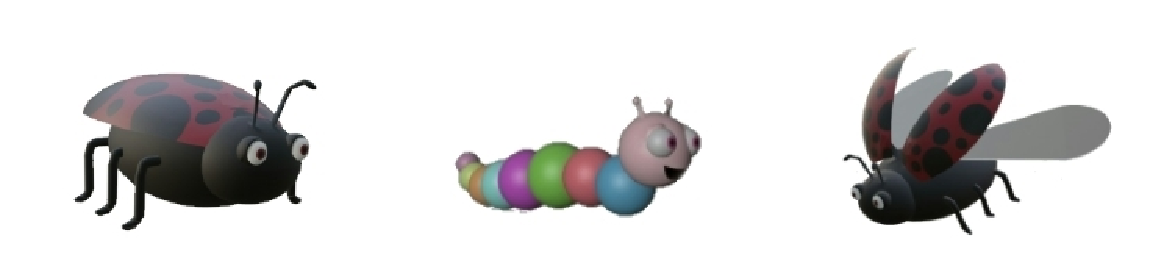
\includegraphics[width=\textwidth]{bugs}
    \caption{Bugs}
    \label{fig:mesh2}
\end{figure}
In addition to traps, the game also features bugs as an obstacle (as shown in Figure \ref{fig:mesh2}). These bugs typically appear in the second tunnel and are designed to align with the player, making them more challenging to evade. However, they can still be avoided by the player. If the player chooses to engage with the bugs, they can be defeated by shooting three bullets at them. If the player collides with a bug, Hans will lose 25\% of his battery life(for more information on battery life, see Section \ref{AdditionalFeatures}).

\subsection{Viruses}
	\begin{figure}[h]
    \centering
    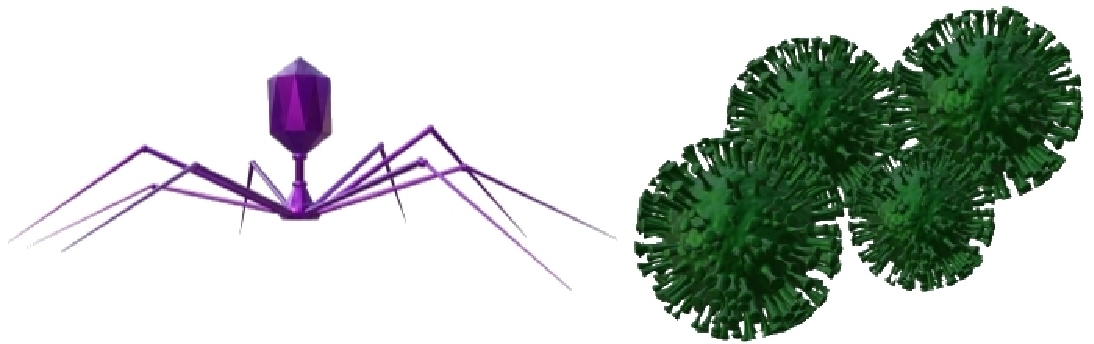
\includegraphics[width=\textwidth]{viruses}
    \caption{Bacteriophage and Rotavirus}
    \label{fig:mesh3}
\end{figure}
The third and final type of obstacle in the game are viruses (illustrated in Figure \ref{fig:mesh3}). These viruses are typically found in the third tunnel and, like bugs, can be eliminated through the use of three bullets. They also align with the player's movement, making them more difficult to evade, although it is still possible to do so. Bacteriophage, a subtype of virus, will result in an instant death if the player comes into contact with them. Rotaviruses, on the other hand, will cause the player's character to become sick for a brief period of time. During this illness, it is crucial for the player to avoid coming into contact with another Rotavirus, as this will result in the end of the game.

\section{Additional Features}
\label{AdditionalFeatures}
There are several other features of the game that are worth mentioning. One of the most significant of these is the battery life of the player's character, Hans, which is displayed on the right side of the screen. As Hans is designed to resemble a computer, it is necessary for him to recharge his battery throughout the game by collecting energy tokens. This will fully restore his battery capacity. There are three main ways in which Hans can lose battery life: running causes a constant reduction of 1\%, each bullet shot costs 1\% of the battery life, and coming into contact with a bug results in a reduction of 25\% (as described in Section \ref{Bugs}). If the battery reaches 0\%, Hans will die and the game will end.

Finally, it should be noted that upon successfully navigating through all three types of tunnels, the game will increase in speed and the player will once again encounter the same tunnels, looping through them indefinitely until the player loses.

\section{Score Count and Winning}
The score of the game is based on the length of time that the player is able to survive. Additionally, each time a player successfully shoots down a bug or virus, their score increases by 10 points. As previously mentioned, the game is designed to be played indefinitely, but for the purpose of this study, we have set the game to be considered won after an agent successfully completes nine tunnels, reaching level 10.

\chapter{Game Implementation}

\section{Title of the first subchapter of the second chapter}

\section{Title of the second subchapter of the second chapter}

\chapter{Structure of the Experimental Setting}
\label{agent_code_chapter}
To train an agent on a specific environment, the user must utilize a command-line interface. There are various options available to cater to the user's needs. This chapter will outline all of the provided options and how they are encoded. However, we will first consider how the game represents discrete states.

\section{State}
The majority of the implemented agents in the game utilize the concept of state to facilitate learning. The agent will determine its next action based on the current state in which it finds itself. By dividing the game into discrete states, we are able to utilize tabular method algorithms to train an agent to play this continuous game. Once one obstacle is passed, the value of the state indicated refers to the next one. Each state is represented by a triplet consisting of distance, rotation, and next obstacle type. 

It is important to note that the game uses meters as the standard unit of distance measurement in Godot. This unit is used to represent the size, position, and movement of objects in the game world. It is worth mentioning that one meter in Godot is equal to the size of a standard cube. With that in mind, players can visualize Hans' approximate height of 12 meters and starting speed of 35 meters per second. Additionally, each tunnel in the game has a width and height of approximately 45 meters and a depth of 2800 meters.

The distance value indicates the distance of the agent from the next obstacle in meters. For example, if we set the \texttt{dists} parameter (indicated by the user, see \ref{opt:dists}) to 2, there are two possible distance values for the state: \textgreater 50, \textgreater 0, indicating that the agent is more than 50 meters away from the obstacle and at least 1-50 meter away from the obstacle, respectively. If the \texttt{dists} parameter is set to 1, the distance value remains constant at \textgreater 0. In the Chapter \ref{experiments_chapter} we will see that all types of environments in this game are able to learn when the \texttt{dists} parameter is equal to 1.  

The rotation parameter divides the obstacle circumference into \texttt{rots} number of intervals (see \ref{opt:rots}). As the tunnel rotates, the state label will indicate the rotation value to which Hans is aligned at the moment (in Figure \ref{fig:circumference} Hans is aligned with rotation value 240). If the \texttt{rots} parameter is set to 360, this would correspond to the number of degrees in a circle and result in 360 possible rotations. However, the obstacles in this game do not require such a high number of rotations and agents can be trained to avoid most obstacles using fewer than 10 rotations. 

\begin{figure}[h]
    \centering
    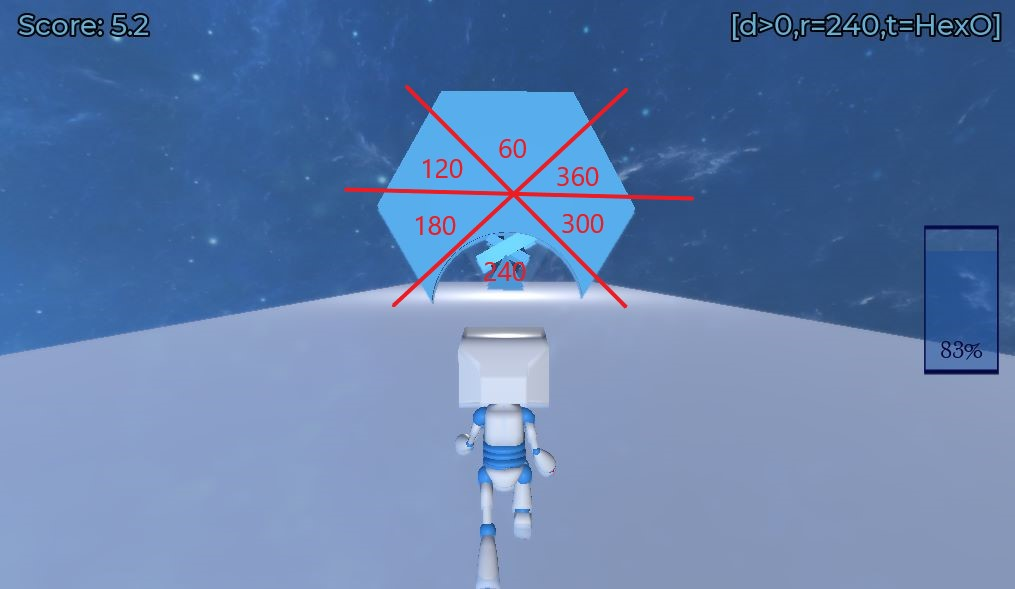
\includegraphics[width=\textwidth]{circumference}
    \caption{Rotations when \texttt{rots = 6}}
    \label{fig:circumference}
\end{figure}

Finally, the type parameter indicates the type of obstacle that Hans must avoid. Each obstacle has its own unique string representation, which allows the agent to learn to recognize the safe rotation for different types of obstacles. Using this information, along with the distance parameter, the agent can decide whether to move left, right, forward, or shoot in combination with any of these actions. To further explain this notion lets look back at the Figure \ref{fig:circumference}. At first glance, it may seem that a rotation of 240 would allow Hans to easily pass through the obstacle. However, upon closer inspection, it becomes clear that only a specific portion of the 240 rotation value is safe. The agent does not know the difference between being at any point of the 240 rotation and thus can easily make a fatal mistake. For this obstacle, indeed, there would be more \texttt{rots} needed in order for Hans to have at least one safe rotation value (meaning that the whole piece of the obstacle that rotation value covers is considered safe).

In Chapter \ref{experiments_chapter}, a noteworthy concept is presented where the agent can recognize a safe edge between two rotations, even if it is not provided with a completely safe rotation. By quickly shifting between these rotations, the agent is able to successfully navigate through the obstacle.

\section{Command line options}
\label{commOpt}
\begin{center}
\resizebox{\textwidth}{!}{%
\begin{tabular}{ | p{4cm}|p{10cm} | } 
  \hline
  \hyperref[opt:n]{n=int} & number of games\\ 
  \hline
  \hyperref[opt:stoppingPoint]{stoppingPoint=int} & stop after the agent wins this many consecutive games\\ 
  \hline
  \hyperref[opt:agent]{agent=string} & name of the agent\\ 
  \hline
  \hyperref[opt:level]{level=int} & number of the level to start from \\ 
  \hline
  \hyperref[opt:env]{env=[string]} & list of obstacles that will be chosen in the game \\ 
  \hline
  \hyperref[opt:shooting]{shooting=string} & enable or disable shooting  \\ 
  \hline
  \hyperref[opt:dists]{dists=int} & number of states in a 100-meter interval \\ 
  \hline
  \hyperref[opt:rots]{rots=int} & number of states in 360 degrees rotation \\ 
  \hline
  \hyperref[opt:agentSeedVal]{agentSeedVal=int} & seed value for the random moves the agent takes\\ 
  \hline
  \hyperref[opt:database]{database=string} & read the data for this command from an existing file and/or update the data after the command is executed  \\ 
  \hline
  \hyperref[opt:ceval]{ceval=bool} & performs continuous evaluation \\ 
  \hline
  \hyperref[opt:debug]{debug=bool} & display debug print statements \\ 
  \hline
  \hyperref[opt:options]{options} & displays options \\ 
  \hline
\end{tabular}}
\end{center}


\subsection{Command line option descriptions}
In this section, a more comprehensive clarification for the table presented earlier is provided. It is important to note that any of the options listed can be left out, as they all have default values assigned to them. In the event that no options are specified, a regular game with the \texttt{Keyboard} agent will be executed.

\subsubsection*{n}
\label{opt:n}
Number of games the agent will train on in this session. The default is 100.

\subsubsection*{stoppingPoint}
\label{opt:stoppingPoint}
If the agents manages to win this many consecutive games, the experiment is stopped. This is used to avoid long experiments if the agent has already learned the right policy and would simply keep winning. The default value is 25.

\subsubsection*{agent}
\label{opt:agent}
Name of the desired agent. \\
Options: [\texttt{Keyboard}, \texttt{Static}, \texttt{Random}, \texttt{MonteCarlo}, \texttt{SARSA}, \texttt{QLearning}, \\ \texttt{ExpectedSARSA}, \texttt{DoubleQLearning}]\\
Sub-options (only for the listed agents):
\texttt{MonteCarlo}, \texttt{SARSA}, \texttt{QLearning}, \texttt{ExpectedSARSA}, \texttt{DoubleQLearning}
=[float, float, float, float] :
[\texttt{gam} (range [0,1]), \texttt{eps} (range [0,1]), \texttt{epsFinal} (range [0,1]), \texttt{initOptVal} (range [0,$\infty$))]\\
Example usage: ``\texttt{agent=MonteCarlo:eps=0.1,gam=0.2}''\\
The meaning of the suboptions is explained in Chapter \ref{applied_algo_chapter}.

\subsubsection*{level}
\label{opt:level}
Number of the level to start from. Default value is 1.\\
Options: \texttt{[1, ... , 15]}\\
Note: after the 15th level, the agent is considered to have won the game.

\subsubsection*{env}
\label{opt:env}
List of obstacles that will be chosen in the game,\\
Options (any subset of): [\texttt{Traps}, \texttt{Bugs}, \texttt{Viruses}, \texttt{Tokens},
\texttt{I}, \texttt{O}, \texttt{MovingI}, \texttt{X}, \texttt{Walls}, \texttt{Hex},
\texttt{HexO}, \texttt{Balls}, \texttt{Triangles}, \texttt{HalfHex},
\texttt{Worm}, \texttt{LadybugFlying}, \texttt{LadybugWalking},
\texttt{Rotavirus}, \texttt{Bacteriophage}]\\
Note: if this parameter is not included, the environment will contain all available obstacles (i.e. the full game).\\
Example usage: ``\texttt{env=HexO,I,Bugs}''\\

\subsubsection*{shooting}
\label{opt:shooting}
Enable or disable shooting.\\
Options: [\texttt{enabled}, \texttt{disabled}, \texttt{forced}]\\
This option is disabled by default or if the environment does not have any bugs or viruses.

\subsubsection*{dists}
\label{opt:dists}
Number of states in a 100-meter interval.\\
This parameter is part of the state label and typical options range from 1 to 3. Default value is 1.

\subsubsection*{rots}
\label{opt:rots}
Number of states in 360 degrees rotation.
This parameter is part of the state label and the minimum viable option is 6. This is also the default value.

\subsubsection*{agentSeedVal}
\label{opt:agentSeedVal}
Seed value for the agent.\\
This parameter is used to produce multiple experiments with different random actions to verify if the agent can really learn under certain conditions or if it simply "to lucky" with the random moves.

\subsubsection*{database}
\label{opt:database}
Read or write data for this command from/to a file.\\
Options: [\texttt{read}, \texttt{write}, \texttt{read\_write}]\\
Note: these files are typically used to start another session of the agent's training from the last point of the previous session, to run a game with visuals and observe the agent's performance, or for plotting the results. This option does not affect the Keyboard, Static, or Random agents. Default option for this parameter is to neither read nor write.

\subsubsection*{ceval}
\label{opt:ceval}
Performs continuous evaluation.\\
This parameter indicates that after each training game, a test game will be played using only the policy(s) learned thus far. For example, if the user specifies ``n=100'', a total of 200 games will be executed, with 100 of them being training games and the remaining 100 being test games. This allows for the assessment of the agent's progress and performance during the training process. 
Options: [\texttt{true},\texttt{false} (default)]

\subsubsection*{debug}
\label{opt:debug}
Display debug print statements.
Options: [\texttt{true},\texttt{false} (default)]

\subsubsection*{options}
\label{opt:options}
Displays all of the mentioned options.


\subsection{Running the program}
There are several possibilities for running the game from the command line. In addition to various combinations of the options listed above, the user has the choice of running an experiment with or without the graphical interface. If they opt for the first possibility, the window will open and the game will be played at its normal speed. On the other hand, if the experiment is run without graphics, it will be over 200 times faster and the output will only be displayed in the terminal. This is achieved by a few things, mainly hiding the CSG geometry in every node. The computational power required to perform union, intersection, etc. on the CSG shapes is quite high and thus by not performing those calculations a game can run much faster. Of course, these shapes are not necessary for the experiments run without graphics, since the collision shapes are the ones that play a role in determining what happened in the game\footnote{The collision shapes refer to the shapes that are used to define the physical bounds of an object for the purpose of collision detection.}.
It is important to acknowledge that the experiments conducted in this study are entirely reproducible owing to the predetermined seed values for all the random variables. However, it should be noted that the values produced by a seed can differ across different versions of the Godot Engine. In order to obtain identical results to the experiments detailed in Chapter \ref{experiments_chapter}, it is recommended to use Godot Engine v3.2.3.stable.

To run the program in the command line, the user may benefit from adding the Godot executable to the PATH environment variable. This will allow them to start the application from the command line simply by entering the command \texttt{godot} while inside the same directory as the \texttt{project.godot} file.

By default, running the program in this manner will launch a normal game with the graphical interface and the \texttt{Keyboard} agent. However, the user can customize their experiment by using a combination of the options listed above. For example:

\begin{algorithm}
\begin{algorithmic}
\State godot database=write agent=SARSA:initOptVal=100.0,eps=0.3 env=HexO n=10 dists=1 rots=8
\end{algorithmic}
\end{algorithm}

Alternatively, the user may choose to train the agent faster by disabling the graphical interface and increasing the speed of the program. This can be achieved by modifying the previous command as follows:

\begin{algorithm}
\begin{algorithmic}
\State godot --no-window --fixed-fps 1 --disable-render-loop database=write agent=SARSA:initOptVal=100.0,eps=0.3 env=HexO n=10 dists=1 rots=8
\end{algorithmic}
\end{algorithm}

To view a list of available options, the user can simply enter the command \texttt{godot options}.

\section{Main}
The \texttt{Main.tscn} scene is the top level scene in the game and consists of a single Node type node. The script attached to this node, \texttt{Main.gd}, is responsible for ensuring that all options specified in the command line (as discussed in Section \ref{commOpt}) are executed correctly. This script is the starting point of the training and handles the initialization and execution of ore or more game sessions.
There are several key functions within the \texttt{Main.gd} script that are worth discussing in more detail.

\begin{algorithm}
\begin{algorithmic}[1]
\Function{\_ready}{}
\State $unparsed\_args \gets OS.\text{get\_cmdline\_args()}$
\If{$unparsed\_args.size() = 1$ and $unparsed\_args[0] = "options"$}
\State \Call{display\_options}{}
\EndIf
\State $\dots$ \Comment{parse args}
\If{\Call{set\_param}{args} $= \text{false}$}
\State \Call{display\_options}{}
\Else
\State \Call{instance\_agent}{}
\State \Call{build\_filename}{}
\If{\textbf{not} $agent\_inst.\text{init}(actions, read, write, command, n, debug)$}
\State \Call{print}{``Something went wrong, please try again''}
\State \Call{display\_options}{}
\EndIf
\State \Call{play\_game}{}
\EndIf
\EndFunction
\end{algorithmic}
\end{algorithm}

The \texttt{\_ready()} function is the starting point of the program when run from the command line. It is responsible for parsing all of the arguments and checking their validity. If any issues are encountered, the program will display options and terminate. If the arguments are valid, an agent will be instantiated and initialized. In cases where everything is in order, first game will be played by calling the \texttt{play\_game()} function.

\begin{algorithm}
\begin{algorithmic}[1]
\Function{play\_game}{}
\If{agent $=$ "Keyboard" and VisualServer.render\_loop\_enabled}
\State $\dots$ \Comment{play a regular game}
\ElsIf{$n > 0$}
\State $n \gets n - 1$
\State $game \gets$ $game\_scene.\text{instance}()$
\State \Call{set\_param\_in\_game()}{}
\State $agent\_inst.\text{start\_game}(is\_eval\_game)$
\Else
\State $agent\_inst.\text{save}(write)$
\State \Call{print\_and\_write\_ending()}{}
\EndIf
\EndFunction
\end{algorithmic}
\end{algorithm}

The \texttt{play\_game()} function is called each time a game is played.Firstly, it will check if the agent selected was the \texttt{Keyboard} agent, and if so, the program will start one game session where the user has controls of Hans. Otherwise, one of the remaining agents will take over and play specified number of games (defined by the "n" parameter). If n games have already been played, the program will terminate after performing the last few tasks needed to save all of the knowledge gained form this particular session. Otherwise, a single game will be executed and number of games left decreased.

\begin{algorithm}
\begin{algorithmic}[1]
\Function{on\_game\_finished}{$score, ticks, win, time$}
    \State \Call{print\_and\_write\_score}{score, win}
    \State $agent\_inst.\text{end\_game}(score, time)$
    \State \Call{play\_game()}{}
\EndFunction
\end{algorithmic}
\end{algorithm}

The \texttt{game\_over()} function is called when the game emits a signal indicating that it has finished. Upon execution, this function outputs the necessary information, updates the agent through the \texttt{end\_game()} function, and then calls the \texttt{play\_game()} function to continue the game session.
\chapter{Applied Algorithms}
In this chapter, we will discuss the algorithms employed to create agents for the game, which broadly fall into the categories of Monte Carlo methods and Temporal Difference (TD) Learning. In essence, the agents aim to maximize their reward by selecting actions that yield the greatest possible benefit. To comprehend the functioning of these algorithms, it is necessary to introduce several fundamental concepts. 

A \textbf{state} represents the current status of the environment, while an \textbf{action} denotes a decision made by the agent in response to the current state. A \textbf{reward} is a scalar value that reflects the immediate feedback received by the agent for its action in a given state. The \textbf{discount factor}, usually denoted as $\bm{\gamma}$, is a value between 0 and 1 that represents how much the agent values future rewards compared to immediate rewards. An \textbf{episode} refers to a sequence of states, actions, and rewards that begins with an initial state and ends when a terminal state is reached. It represents one run or iteration of the agent interacting with the environment. The length of an episode can vary depending on the problem and the algorithm being used (eg. in a game, an episode may correspond to a single game). A \textbf{policy} is a mapping from states to actions that determines the actions an agent takes in each state. An \textbf{$\bm{\epsilon}$-greedy policy} is a policy in which the agent selects the action that maximizes the expected reward with a probability of (1 - $\epsilon$), while taking a random action with a probability of $\epsilon$. Two types of value functions exist, namely \textbf{state-value} functions and \textbf{action-value} functions. The former predict the expected long-term reward of being in a particular state, while the latter predict the expected long-term reward of taking a specific action in a particular state and always following the optimal policy thereafter. The value function evaluates the relative effectiveness of different actions or states, serving as a measure to determine the optimal action in a particular state. The \textbf{value of a state} varies between algorithms, and it is used to select the best action to be taken in that state. 

Before looking into individual algorithms, there is one more key concept to introduce: \textbf{exploration vs exploitation}. In the field of reinforcement learning, the exploration-exploitation trade-off refers to the balancing act between discovering new information or strategies and utilizing existing knowledge to maximize reward. Exploration involves trying out different actions or strategies in order to gather more information about the environment and its rewards, while exploitation involves utilizing the information gathered to maximize reward. Finding the right balance between exploration and exploitation is crucial in reinforcement learning, as excessive use of either can result in suboptimal results. To balance out these two concepts within these algorithms two methods are used: the formerly mentioned \textbf{$\bm{\epsilon}$-greedy policy} as well as the \textbf{optimistic initial values} which is a technique which sets the initial value of all state action pairs to a high number, encouraging the agent to visit as many states as possible in order to learn their true value \citep{RLSuttonBarto}.

\section{Monte Carlo}
Monte Carlo (MC) methods are a type of reinforcement learning algorithm that estimate the value of a state or action by averaging the total reward received from sample episodes. Unlike some other methods, such as dynamic programming, MC methods do not require knowledge of the transition probabilities between states or the reward function. Instead, they learn from experience by directly observing the outcomes of sample episodes.

During each episode, the agent follows its policy to select actions, receives rewards from the environment, and transitions to the next state. Once an episode terminates, the total reward received from that episode is recorded. This total reward is used to update the value estimates for each state and action that were encountered during the episode.

There are two types of MC learning: on-policy and off-policy. On-policy learning means that the agent is using the same behavior policy to collect samples as it is using to improve the value function. Off-policy learning, on the other hand, means that the agent is using a different policy to collect samples than the policy it is using to improve the value function.

One variant of on-policy MC learning is first visit Monte Carlo. This method only considers the first time a state is visited in an episode, as opposed to all visits. The goal of using this method is to reduce variance in the value estimates and improve learning efficiency.

To ensure exploration during learning, the $\epsilon$-greedy policy is often used in conjunction with MC methods. Additionally, setting an initial optimistic value can encourage the agent to visit more states to learn their true values. While Monte Carlo methods are guaranteed to converge to an optimal policy with an infinite number of samples, convergence can be slow and estimates can be noisy (i.e., have high variance) with a small number of samples.

The pseudocode for the first-visit Monte Carlo can be seen in Algorithm \ref{algo:MC} \citep{RLSuttonBarto}.

\begin{algorithm}
\caption{On-policy first-visit Monte Carlo}\label{algo:MC}
\begin{algorithmic}[1]
\State Initialize
\State $\quad$ $V(s) \gets$ an arbitrary value for all $s \in \mathcal{S}$
\State $\quad$ $Returns(s) \gets 0$ for all $s \in \mathcal{S}$
\State Loop forever (for each episode):
\State $\quad$ Generate an episode following policy $\pi$
\State $\quad$ $G \gets 0$
\State $\quad$ Loop for each step of episode, $t=T-1,T-2,\ldots,0$:
\State $\qquad$ $G \gets \gamma G + R_{t+1}$
\State $\qquad$ If $S_t$ not in $S_0,S_1,\ldots,S_{t-1}$:
\State $\qquad\quad$ $Returns(S_t) \gets Returns(S_t) + 1$
\State $\qquad\quad$ $V(S_t) \gets V(S_t) + \frac{(G-V(S_t))}{Returns(S_t)}$
\end{algorithmic}
\end{algorithm}

To clarify the algorithm above, here are further explanations to some of the elements mentioned:
\begin{itemize}
\item S - The set of all possible states.
\item V(s) - The estimated value of a state s, i.e., the expected return that the agent will receive by starting from state s and following the current policy thereafter. In other words, V(s) is the agent's prediction of how good it is to be in state s.
\item Returns(s) - The list of returns that the agent has observed from state s during the course of multiple episodes. Each element in the list represents the total reward that the agent received from a single episode that started in state s.
\item G - The actual total return that the agent received from a single episode that started in state s. In other words, it is the sum of all the rewards that the agent received from the start state until the end of the episode.
\end{itemize}

In Chapter \ref{implOfAgents} of this work, we will provide a detailed discussion of the specific Monte Carlo algorithm implementation employed. Furthermore, we will explain how  the initial optimistic value and $\epsilon$-greedy policy have been utilized in the algorithm.

\section{Temporal Difference Learning}
Temporal Difference (TD) learning is another type of reinforcement learning algorithm that is also model-free. The main idea behind it is to update the estimated value of a state or action based on the difference between the expected return and the actual return obtained from that state or action. 

TD learning is similar to Monte Carlo methods in that it learns from experience by interacting with the environment and observing the rewards received. However, these methods update their estimates after every time step, rather than waiting for an entire episode to complete like in MC methods. This makes Temporal Difference learning more efficient in terms of the amount of data needed to learn a good estimate of the value function.

Like Monte Carlo methods, TD methods can also be on-policy or off-policy. In on-policy learning, the agent learns about the value of the policy it is currently following, whereas in off-policy learning, the agent learns about the value of a different policy. 

One important parameter in TD learning is the \textbf{step size} or \textbf{learning rate} (usually denoted by the symbol $\bm{\alpha}$), which determines the size of the update to the value estimates. A larger step size will result in faster learning, but may also make the learning process more unstable.

In this chapter, we shall introduce four distinct TD learning algorithms, namely SARSA, Q-Learning, Expected SARSA and Double Q-Learning. We shall illustrate that while SARSA and Q-Learning are prominent algorithms for control problems, Expected SARSA and Double Q-Learning are variations that cater to specific limitations of the original algorithms. The objective is to highlight both the commonalities and differences among them.

\subsection{SARSA}
SARSA stands for State-Action-Reward-State-Action. With this algorithm, the agent learns the value of a state-action pair Q(s,a) by estimating the expected return of starting from state s, taking action a, and then following the current policy. SARSA is an on-policy algorithm, meaning it learns the value of state-action pairs while following the same policy used to select actions. This makes it well-suited for control problems, where the goal is to find an optimal policy.
\begin{algorithm}
\caption{SARSA}\label{algo:S}
\begin{algorithmic}[1]
\State Initialize $Q(s,a)$ arbitrarily for all $s\in S$ and $a\in A(s)$
\Repeat
\State Choose $A$ from $S$ using policy derived from $Q$ (e.g., $\epsilon$-greedy)
\Repeat
\State Take action $A$, observe $R$, $S'$
\State Choose $A'$ from $S'$ using policy derived from $Q$ (e.g., $\epsilon$-greedy)
\State $Q(S,A) \gets Q(S,A) + \alpha \big[ R + \gamma Q(S',A') - Q(S,A) \big]$
\State $S \gets S'$
\State $A \gets A'$
\Until $S$ is terminal
\Until convergence
\end{algorithmic}
\end{algorithm}

\subsection{Q-learning}
Q-learning, unlike SARSA, is an off-policy algorithm that learns the value of a state-action pair Q(s,a) by estimating the maximum expected return over all possible actions from state s. In other words, it learns the value of the best action in each state. Since Q-learning is an off-policy algorithm that learns the optimal action-value function regardless of the current policy being followed. This makes Q-learning more flexible in terms of exploration and can result in faster convergence to the optimal policy. However, Q-learning tends to overestimate the value of actions in environments with high variance, which can lead to suboptimal policies. On the other hand, SARSA is more stable and less prone to overestimating the value of actions. Nevertheless, it can converge to suboptimal policies if the exploration is insufficient, and it can take longer to converge to the optimal policy compared to Q-learning.
\begin{algorithm}
\caption{Q-learning}\label{algo:QL}
\begin{algorithmic}[1]
\State Initialize $Q(s,a)$ arbitrarily for all $s \in S$ and $a \in A(s)$.
\Repeat
\Repeat
\State Choose $A$ from $S$ using policy derived from $Q$ (e.g., $\epsilon$-greedy).
\State Take action $A$, observe $R$, $S'$
\State $Q(S,A) \gets Q(S,A) + \alpha \left[R + \gamma \max_a Q(S',a) - Q(S,A)\right]$
\State $S \gets S'$
\Until $S$ is terminal
\Until convergence
\end{algorithmic}
\end{algorithm}

\subsection{Expected SARSA}
Expected SARSA is another off-policy TD algorithm that learns the value of a state-action pair Q(s,a) by estimating the expected return over all possible actions from state s, taking into account the probabilities of selecting each action according to the current policy. Expected SARSA can be seen as a compromise between SARSA and Q-learning, as it considers the value of both the current and the best action in each state. This algorithm considers all possible actions and their expected values, which makes it more robust to noisy or uncertain rewards. 
\begin{algorithm}
\caption{Expected SARSA}\label{algo:ES}
\begin{algorithmic}[1]
\State Initialize $Q(s,a)$ arbitrarily for all $s \in S$ and $a \in A(s)$
\Repeat \textbf{for each episode:}
\State Initialize $S$
\Repeat \textbf{for each step of episode:}
\State Choose $A$ from $S$ using policy derived from $Q$ (e.g., $\epsilon$-greedy)
\State Take action $A$, observe $R$, $S'$
\State $\text{expected}Q \gets \sum{a} \pi(S',a) Q(S',a)$
\State $Q(S,A) \gets Q(S,A) + \alpha \cdot [R + \gamma \cdot \text{expected}_Q - Q(S,A)]$
\State $S \gets S'$
\Until $S$ is terminal
\Until convergence
\end{algorithmic}
\end{algorithm}


\subsection{Double Q-learning}
Double Q-learning is a variant of Q-learning that uses two action-value functions to estimate the value of each action. The two functions are updated independently, and the final action-value estimate is the average of the two estimates. In Q-Learning, a single estimate of the action values is used to update the policy and make decisions. This can lead to overestimation of the action values, particularly in situations where the policy is still exploring the environment. Double Q-Learning addresses the overestimation issue in Q-Learning which can lead to more accurate value estimates and better performance in some cases.
\begin{algorithm}
\caption{Double Q-learning}\label{algo:DQL}
\begin{algorithmic}[1]
\State Initialize $Q_1(s,a)$ and $Q_2(s,a)$ arbitrarily for all $s \in S$ and $a \in A(s)$
\For {each episode}
\State Initialize $S$
\For {each step of episode}
\State Choose $A$ from $S$ using policy derived from $Q_1+Q_2$ (e.g., epsilon-greedy)
\State Take action $A$, observe $R$, $S'$
\If {rand() $<$ 0.5}
\State $A' \gets \text{argmax}_a Q_1(S',a)$
\State $Q_1(S,A) \gets Q_1(S,A) + \alpha [R + \gamma Q_2(S',A') - Q_1(S,A)]$
\Else
\State $A' \gets \text{argmax}_a Q_2(S',a)$
\State $Q_2(S,A) \gets Q_2(S,A) + \alpha [R + \gamma Q_1(S',A') - Q_2(S,A)]$
\EndIf
\State $S \gets S'$
\EndFor
\State until $S$ is terminal
\EndFor
\end{algorithmic}
\end{algorithm}
\chapter{Implementation of the Agents}
\label{implOfAgents}
In this project, the reinforcement learning (RL) agents agents are designed such that their functionality is encapsulated within a top-level scene called \texttt{Main.tscn}. Within this scene, there is an instance of the selected agent, and the code makes use of several functions implemented by the agent in order to interact with the environment. Specifically, the required functions include: \texttt{move()}, \texttt{init()}, \texttt{start\_game()}, \texttt{end\_game()}, \texttt{save()}.

The purpose of most of these functions is self-explanatory. \texttt{init()} and \texttt{save()} are used to initialize and save the agent's internal state, respectively, and are called only once per experiment. \texttt{start\_game()} and \texttt{end\_game()} are called at the beginning and end of each episode, while \texttt{move()} is called by the \texttt{Tunnels.gd} script, and it is in this function that the agent makes a decision about which action to take based on the current state and score.

\section{Hierarchy}
\begin{figure}[h]
    \centering
    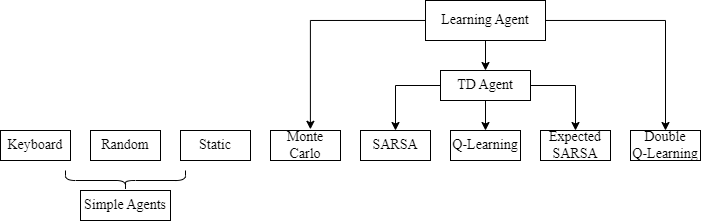
\includegraphics[width=0.8\textwidth]{agents_tree}
    \caption{Agents hierarchy inside the project}
    \label{fig:agents_tree}
\end{figure}

In the current design of the game, there are a total of 8 agents implemented, 5 of which utilize some form of reinforcement learning algorithm. These RL agents share a common superclass called \texttt{LearningAgent}, while 3 of them are further subclassed under the \texttt{TDAgent} class (see Figure \ref{fig:agents_tree}). As previously discussed, the RL algorithms can be broadly divided into two categories: Monte Carlo methods and temporal difference (TD) learning. The TD algorithms differ only in their update function, and so it was deemed appropriate to group them under the same superclass. However, the Double Q-Learning agent, which uses separate policies and requires additional modifications, was implemented as a separate subclass of the \texttt{LearningAgent}. The implementation details of these agents will be further elaborated upon in the subsequent sections. 

As previously mentioned when describing the state in Chapter 3, the agent has the ability to perform movements in various directions, including moving right, forward, or left, and each of these movements can be performed in combination with shooting. Therefore, on each time step, the move function of the agent returns a list of two elements: the first element signifies the movement direction, where a value of -1 represents left, 0 represents forward, and 1 represents right; while the second element determines whether the agent will shoot or not, with a value of 1 indicating yes and 0 indicating no for shooting.


\section{Simple Agents}
To facilitate testing of the game environment, several simple agents were implemented. These agents serve as baseline models and were used to ensure that the environment was functioning as intended before more sophisticated RL agents were developed. There are three simple agents in total: a ``Keyboard agent'' that receives input from the player via the keyboard, a ``Static agent'' that always chooses the forward action without shooting, and a ``Random agent'' that chooses a random action at each time step. 

\section{Learning Agent}
This class serves as a base class for all the reinforcement learning agents in this project. It provides a set of shared functions and features that are used by all agents, such as reading and writing data to a file and debugging statements. In terms of decision-making, these agents all follow an $\epsilon$-greedy policy, whereby they select the action with the highest value for a given state with a certain probability, or randomly choose any action with the remaining probability. Each of the subclasses of the \texttt{LearningAgent} class then implements specific code that is unique to that particular agent.

\begin{center}
\hrulefill
\begin{lstlisting}
func choose_action(action):
    epsilon_action = false
    if not is_eval_game: # Used for continuous evaluation
        epsilon_action = rand.randf_range(0,1) < EPSILON
        if epsilon_action:
            action = ACTIONS[rand.randi\_range(0,len(ACTIONS) - 1)]  
    return action
\end{lstlisting}
\hrulefill
\end{center}

\subsection{Common parameters and behaviours}
In regards to the present implementation of the reinforcement learning algorithms for the 3D tunnel game, certain aspects of the game learning step and parameter implementation are unique to this project and merit discussion. For instance, we should look into the learning step in the game. The agent will not request a new move until the state has changed, despite the fact that it may seem more natural for a new decision to be made on every game tick. This has the effect of reducing the number of decisions that the agent must make in a given episode, but also results in intriguing policy behaviours that are elaborated upon in Chapter \ref{experiments_chapter}.

Furthermore, there are several parameters that are common to all learning agents, some of which were briefly discussed in the preceding chapter. In this section, we will examine in more detail how these parameters were integrated into this particular project. The initial optimistic value parameter is the simplest one to explain, as it is implemented in a straightforward manner. In particular, each time a state-action pair is added to the policy, its value is set to a predetermined number. This number (\texttt{initOptVal}), along with the other agent's sub-options parameters mentioned subsequently in this subsection, are specified through the command line (see \ref{commOpt}).

The following two parameters worth noting are \texttt{eps} and \texttt{epsFinal}, which are responsible for the random moves executed by the $\epsilon$-greedy policy. These parameters allow the user to specify the starting and ending values of $\epsilon$. Then, at the end of each game, the new $\epsilon$ value is calculated by multiplying the current $\epsilon$ value with the $decrease$ which is computed as follows\footnote{This computation is performed once, when initializing the agent.}: $$decrease = (\frac{epsFinal}{eps})^{\frac{1.0}{n}}$$

Here, \texttt{n} represents the number of games being played. The reason behind this epsilon decrease is to change the ratio between exploration and exploitation over time. At the beginning of the experiment, the \texttt{eps} value is higher, and thus random moves happen more often, causing the agent to try actions it would otherwise oversee. Later, when the policy is a bit stabilized, the \texttt{eps} value becomes smaller so it would allow the agent to play longer games and possibly win (if the \texttt{eps} value was high throughout the whole experiment, the agent would have a bigger chance of choosing an inadequate move and thus untimely ending the game).

Finally, it is pertinent to discuss the discounting value $\gamma$ (defined by \texttt{gam}). In this project, discounting is used in the following manner: $$\gamma^{next\_step.time - curr\_step.time}$$

In many reinforcement learning environments, all learning steps have the same duration, so each reward is discounted by $\gamma^{n}$, where \texttt{n} is the number of steps that elapsed between the time when an action was taken and the time when the reward was received.  And so in a typical implementation that iterates over the steps in an episode, the accumulated discount rate is multiplied by $\gamma$ in each iteration. However, as previously stated, learning steps in this implementation do not occur on every tick, but instead occur when the state changes. As a result, they may vary in size. To avoid uneven discounting, the time (in milliseconds) is calculated for each new decision made by the agent using this formula:  $$(game.num\_of\_ticks * 33) / 1000.0$$

\subsection{Monte Carlo Agent}

\begin{center}
\hrulefill
\begin{lstlisting}
# MonteCarlo agent update
var R = (next_step.score - curr_step.score)
G = pow(GAMMA,next_step.time - curr_step.time) * (R + G)
            
# since we are using the first visit approach,
# we only need the first occurrence  of this state_action
if is_first_occurrence (...):
    total_return[curr_step.state_action] += G
    visits[curr_step.state_action] += 1
\end{lstlisting}
\hrulefill
\end{center}

The Monte Carlo method is a type of reinforcement learning algorithm that updates its policy only after an episode is completed. This is done by iterating through the entire episode, going from the last step towards the first, and increasing the number of visits and total return for each state-action pair, if this is their first visit inside this episode. The total return is calculated using the formula shown in the code above, while the number of visits is simply incremented by 1. To determine the optimal action, the agent compares the ratio of total return to number of visits for each possible action at a given state\footnote{The pseudocode in Algorithm \ref{algo:MC} keeps a list of all returns for each state/action pair, while in our implementation a return for a particular state/action pair is calculated with the mentioned ratio.}. This calculation is performed at each state transition during the episode. To clarify, instead of calculating a new move each time the \texttt{move()} function is called, the agents will always choose the same action based on the current state. Only once the state has changed, the new action is chosen based on the accumulated score and the new state. This implementation has resulted in a certain behaviour of the agents which will be more discussed in Chapter \ref{intbeh}.
As previously mentioned, the $\gamma$ constant in the equation shown in the code serves as a discount factor, meaning that the last move made, which resulted in termination of the game, will receive the highest penalty. As we move further down the list of moves, their significance decreases. It is important to note that if the value of $\gamma$ is set to 1, all moves are given equal weight. 

\subsection{TD Agent}	
Unlike the Monte Carlo methods, which update their policies only after the completion of an episode, TD agents update their policies in real time, after each action is taken. To accomplish this, all TD agents have a shared function called \texttt{move()}, which calls the function displayed in the code provided below. 

\begin{center}
\hrulefill
\begin{lstlisting}
# TD agents update
visits[last_state_action] += 1
var alpha = 1.0 / visits[las\t_state_action]
var new_stat\e_val = 0 if terminal else new_state_action
var new_gamma = pow(GAMMA,curr_time - prev_time)
q[last_state_action] += alpha * (new_gamma * (R + new_state_val) - q[last_state_action])
\end{lstlisting}
\hrulefill
\end{center}

The update of the policy for a specific state value in TD learning involves multiple variables, most of which have been previously discussed. One new variable is $\alpha$, which represents one devided by the total number of visits for a given state action pair. Furthermore, to make this calculation, a variable uniquely computed by each TD algorithm, known as \texttt{new\_state\_action}, is required. Various methods for computing this variable can be found in the code-snippets below. If the current state is a terminal state, the \texttt{new\_state\_action} will not be used and instead, it will be replaced with a value of 0, as indicated in the update code.

\begin{center}
\hrulefill
\begin{lstlisting}
# SARSA agent new_state_action variable calculation
func get_update(state, new_action, _best_action):
    return q[get_state_action(state, new_action)]
\end{lstlisting}
\hrulefill
\end{center}

\begin{center}
\hrulefill
\begin{lstlisting}
# QLearning agent new_state_action variable calculation
func get_update(state, _new_action, best_action):
    return q[get_state_action(state, best_action)]
\end{lstlisting}
\hrulefill
\end{center}

\begin{center}
\hrulefill
\begin{lstlisting}
# ExpectedSARSA agent new_state_action variable calculation
func get_update(state, _new_action, best_action):
    var sum = 0.0 
    for action in ACTIONS:
        var probability = EPSILON / len(ACTIONS)
        if action == best_action:
            probability += 1 - EPSILON
        sum += probability * Q(state,action)
    return sum
\end{lstlisting}
\hrulefill
\end{center}

In SARSA, the \texttt{new\_state\_val} is calculated based on the value of the next action the agent will take, denoted as \texttt{new\_action}. On the other hand, Q-learning uses the value of the best action possible in the next state, denoted as \texttt{best\_action}. These two variables are equal if a greedy policy is implemented. However if we consider a $\epsilon$-greedy policy, then they might differ based on whether a random action has been chosen. Expected SARSA combines these two approaches by taking the expected value of all possible actions in the next state. 

\begin{center}
\hrulefill
\begin{lstlisting}
# DoubleQLearning agent update
visits[last_state_action] += 1
var alpha = 1.0 / visits[last_state_action]
var new_gamma = pow(GAMMA, curr_time - prev_time)

if rand.randf_range(0,1) < 0.5:
    var new_state_val = 0 if terminal else
        q2[get_state_action(state,.best_action(state,q))]
    q[last_state_action] += alpha * (new_gamma * (R + new_state_val) -q[last_state_action])
else:
    var new_state_val = 0 if terminal else
        q[get_state_action(state,.best_action(state,q2))]
    q2[last_state_action] += alpha * (new_gamma * (R + new_state_val) -q2[last_state_action])
\end{lstlisting}
\hrulefill
\end{center}

Similar to the agents in the TD class, the update for the Double Q-Learning agent occurs each time the agent changes its state. The update process is slightly different. In this method, two separate action-value functions, denoted as Q1 and Q2, are used to estimate the maximum action value for a given state. At each update step, one of the Q-values is selected randomly and updated using the other Q-value as a reference. This process helps to reduce the overestimation of action values and leads to more stable learning.
\chapter{Experiments}
\label{experiments_chapter}
In this chapter, we will evaluate the performance of the various agents when confronted with different combinations of obstacles, as well as presenting interesting observations made during the experiments. One of the key questions we aim to answer is whether any of the agents are a are capable of learning to play the entire game.

\section{Individual traps environments}
This section discusses the performance of agents in environments containing only one trap at a time.

\begin{figure}[h]
    \centering
    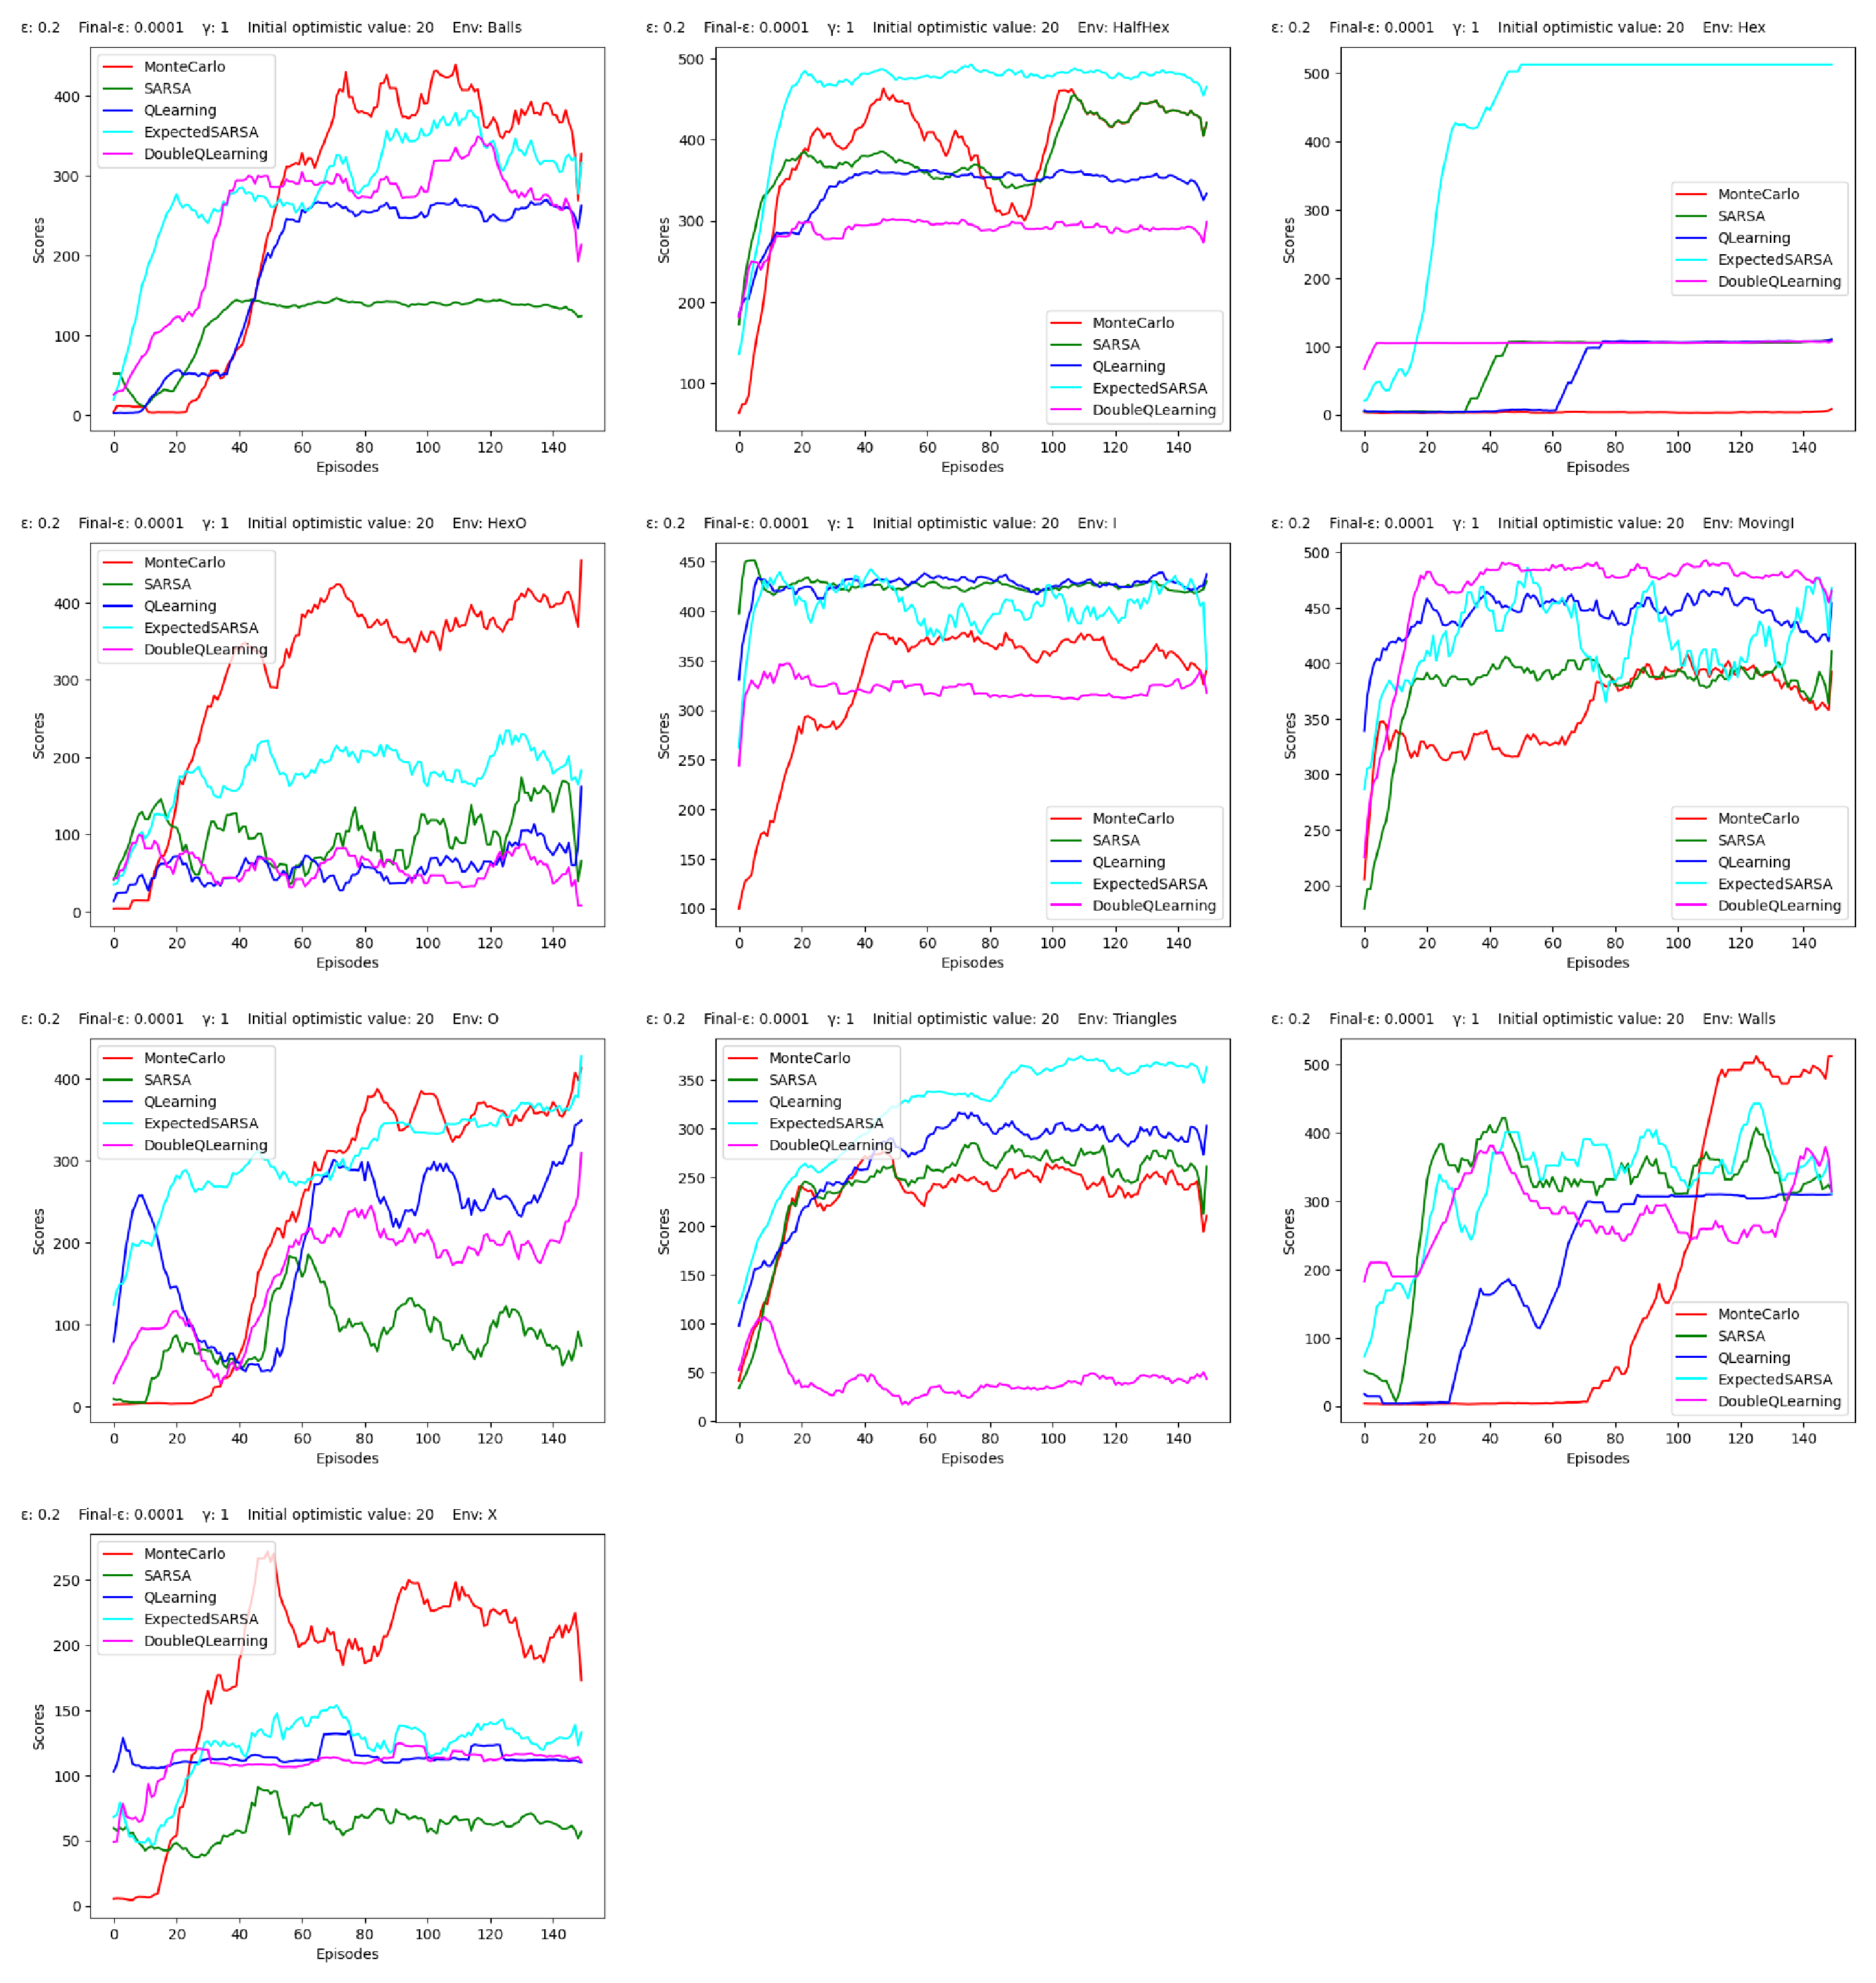
\includegraphics[width=\textwidth]{all_traps}
    \caption{Individual traps examples}
    \label{fig:all_traps}
\end{figure}

Immediately in Figure \ref{fig:all_traps}, for each trap, there is a plot with \texttt{eps=0.2} and \texttt{initOptVal=20} and how each agent performed in this case. These values were picked because with most traps the agents performed well under these conditions.

It should be noted that all plots within this section have smoothing applied with \texttt{window=10}. Thus certain spikes are not be visible. Additionally, unless otherwise suggested, you can assume that the values that were produced are an average of 5 different seeds. The aim is to show a realistic picture on how the agent would perform, and not show the occurrences in which the outcome was satisfactory but rather account for the failures in reproducing the perfect policy as well.

In some cases, of course, the hyperparameters used for plotting Figure \ref{fig:all_traps} were not ideal. However, for most trap/agent pairs, we managed to find at least one combination of hyperparameters where the agent found an optimal or decent policy across multiple seeds. The only exceptions were the \texttt{MonteCarlo} agent with the \texttt{Hex} trap, \texttt{DoubleQLearning} with \texttt{HexO}, \texttt{Triangles}, and \texttt{X} traps, and \texttt{SARSA} and \texttt{QLearning} with \texttt{HexO} trap. \texttt{ExpectedSARSA} was the only agent that produced satisfactory results for all individual trap types and even performed exceptionally well with certain hyperparameters for the \texttt{Hex}, \texttt{I}, \texttt{MovingI}, \texttt{O}, and \texttt{Walls} traps, in which cases it found an optimal policy across multiple seed values.

\begin{figure}[h]
    \centering
    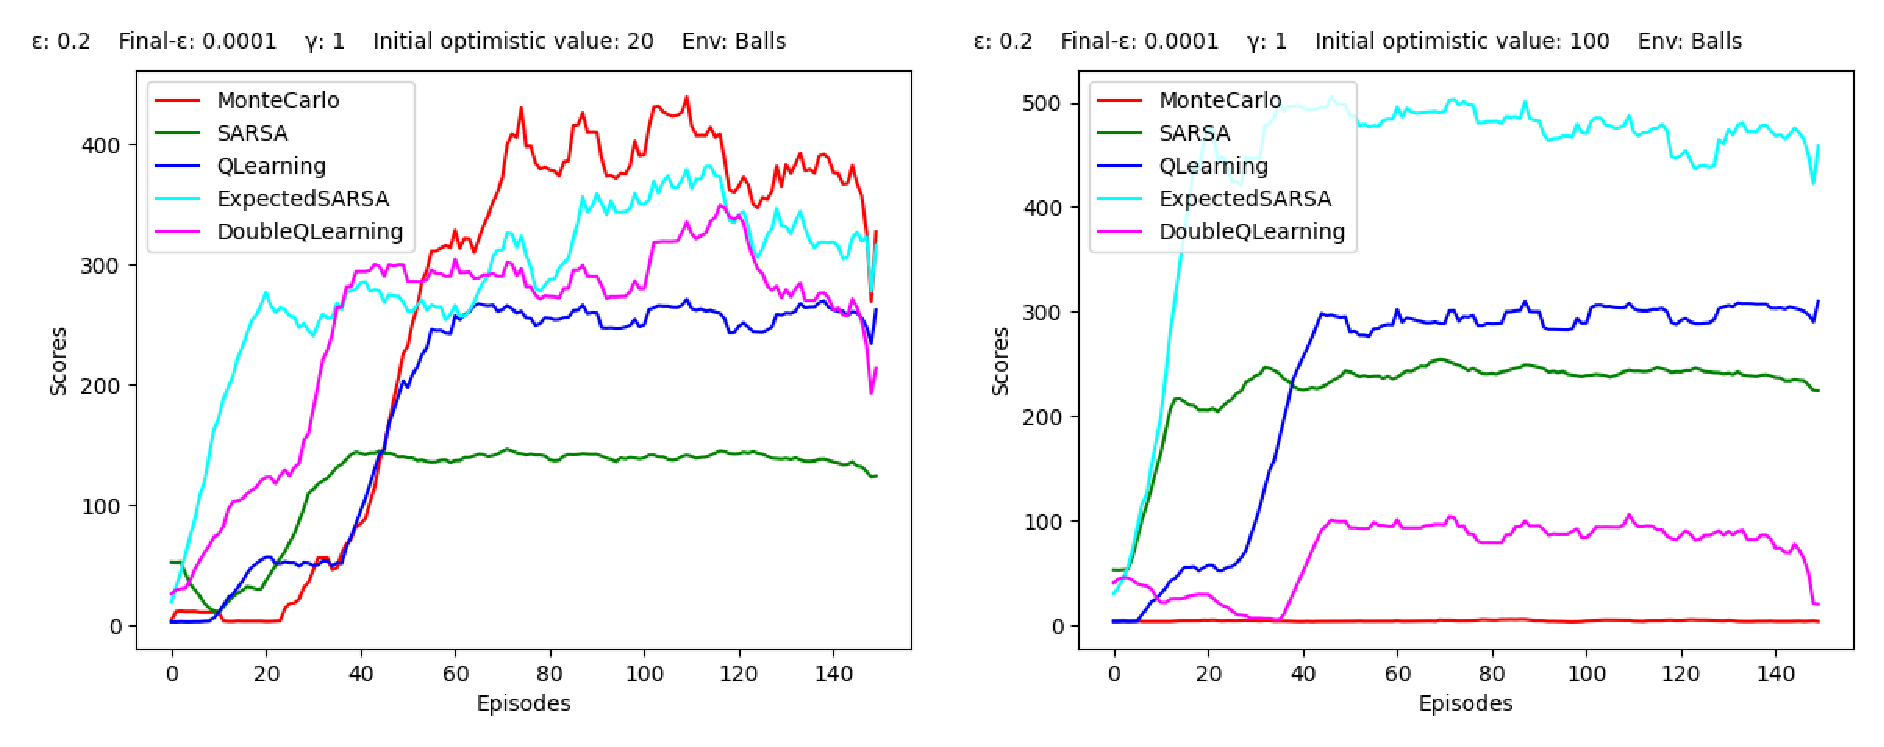
\includegraphics[width=\textwidth]{balls}
    \caption{\texttt{Balls} trap examples}
    \label{fig:balls_eg}
\end{figure}

Choices of the hyperparameters are a very important factor. Most the commonly values in this section are \texttt{eps=0.2} and \texttt{initOptVal=20.0}\\ or \texttt{initOptVal=100.0}. A good example of how much hyperparameters can influence the outcome visible in Figure \ref{fig:balls_eg}. The \texttt{Balls} trap varies significantly based on the initial optimistic value used. This plot underscores the importance of carefully selecting hyperparameters when training reinforcement learning.

\begin{figure}[h]
    \centering
    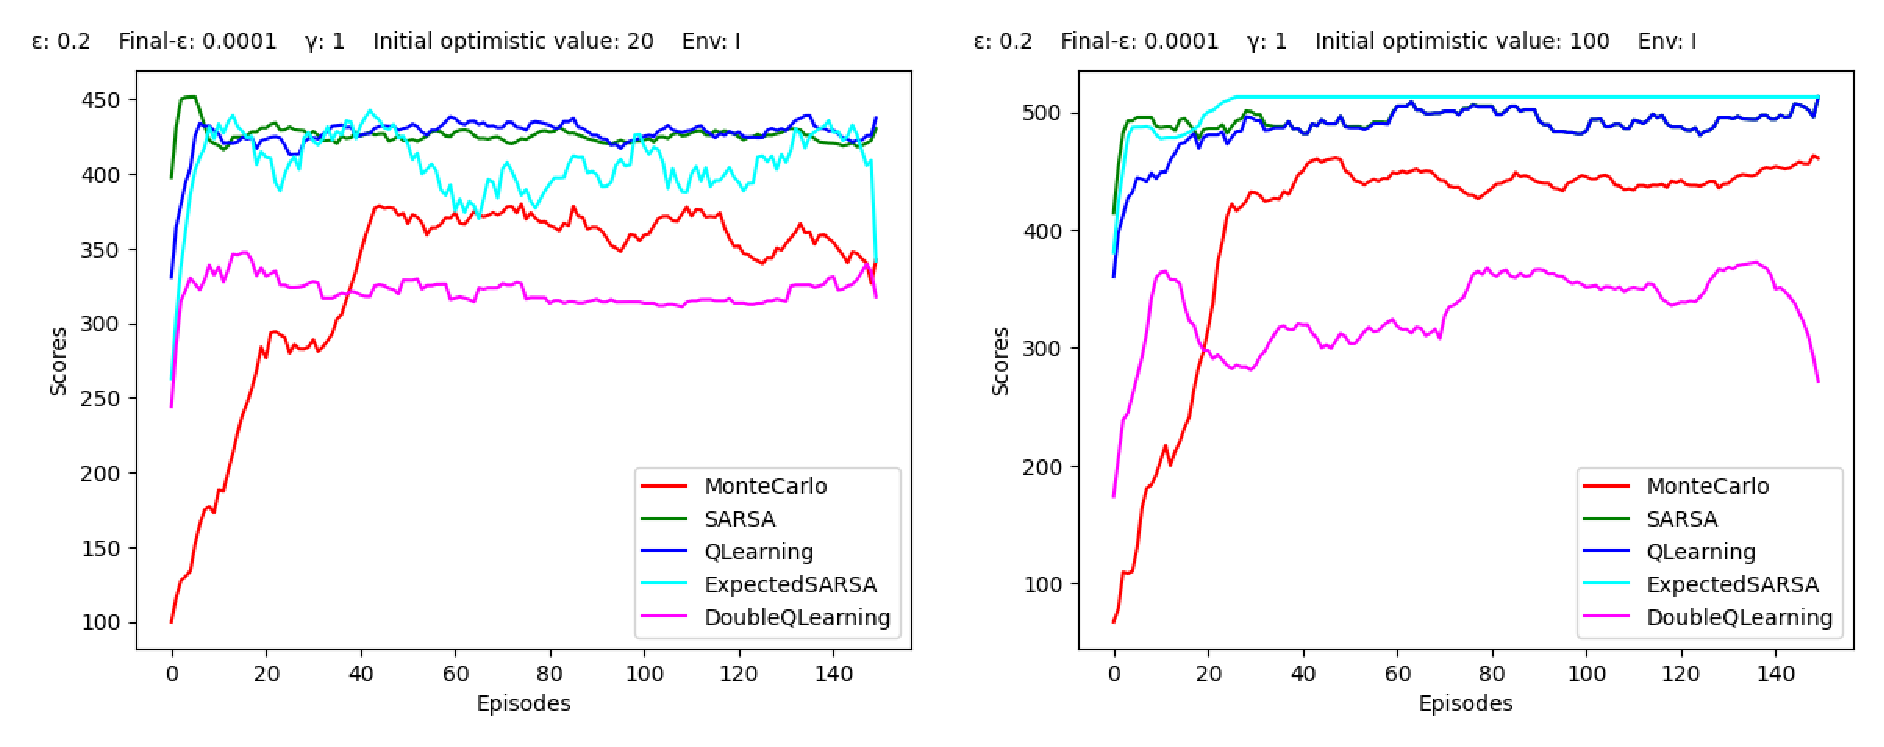
\includegraphics[width=\textwidth]{i}
    \caption{\texttt{I} trap examples}
    \label{fig:i_eg}
\end{figure}

\begin{figure}[h]
    \centering
    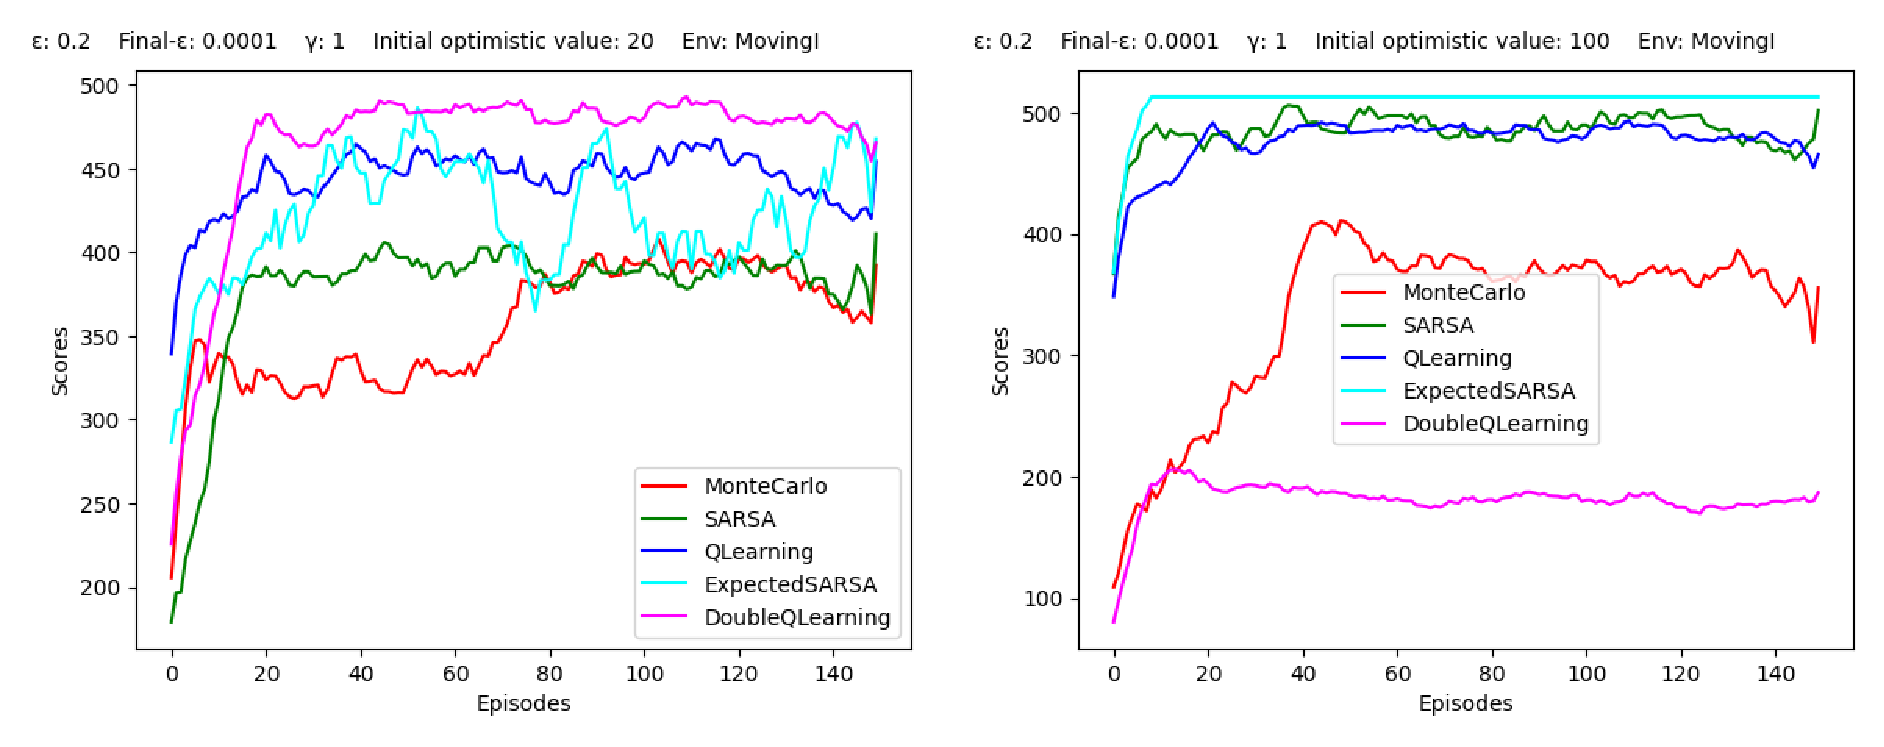
\includegraphics[width=\textwidth]{movingi}
    \caption{\texttt{MovingI} trap examples}
    \label{fig:movingi_eg}
\end{figure}

It is worth noting that there exist cases where the aforementioned variations in hyperparameter selection lead to highly desirable outcomes. This is exemplified by the results presented in Figures \ref{fig:i_eg} and \ref{fig:movingi_eg}, which demonstrate the efficacy of the \texttt{ExpectedSARSA} agent. Notably, on the right hand side of the both plots, the \texttt{ExpectedSARSA} agent was able to achieve optimal performance early on in the game with all seed values. \texttt{ExpectedSARSA} agent, in a very large number of experiments, has outperformed its counterparts, sometimes by a significant amount. This is particularly evident when considering its performance in simpler environments such as traps \texttt{I} and \texttt{MovingI}, where it is apparent that the agent is capable of learning extremely well. While other agents have performed well on these specific traps as well, their success may not be immediately apparent from the averaged results depicted in the plots.

Although performing these experiments with a larger number of seeds would ideally yield even more accurate results, we hope that the picture we presented provides a reasonable representation of the agents' performance in the demonstrated environments.

\section{Traps environment}
\begin{figure}[h]
    \centering
    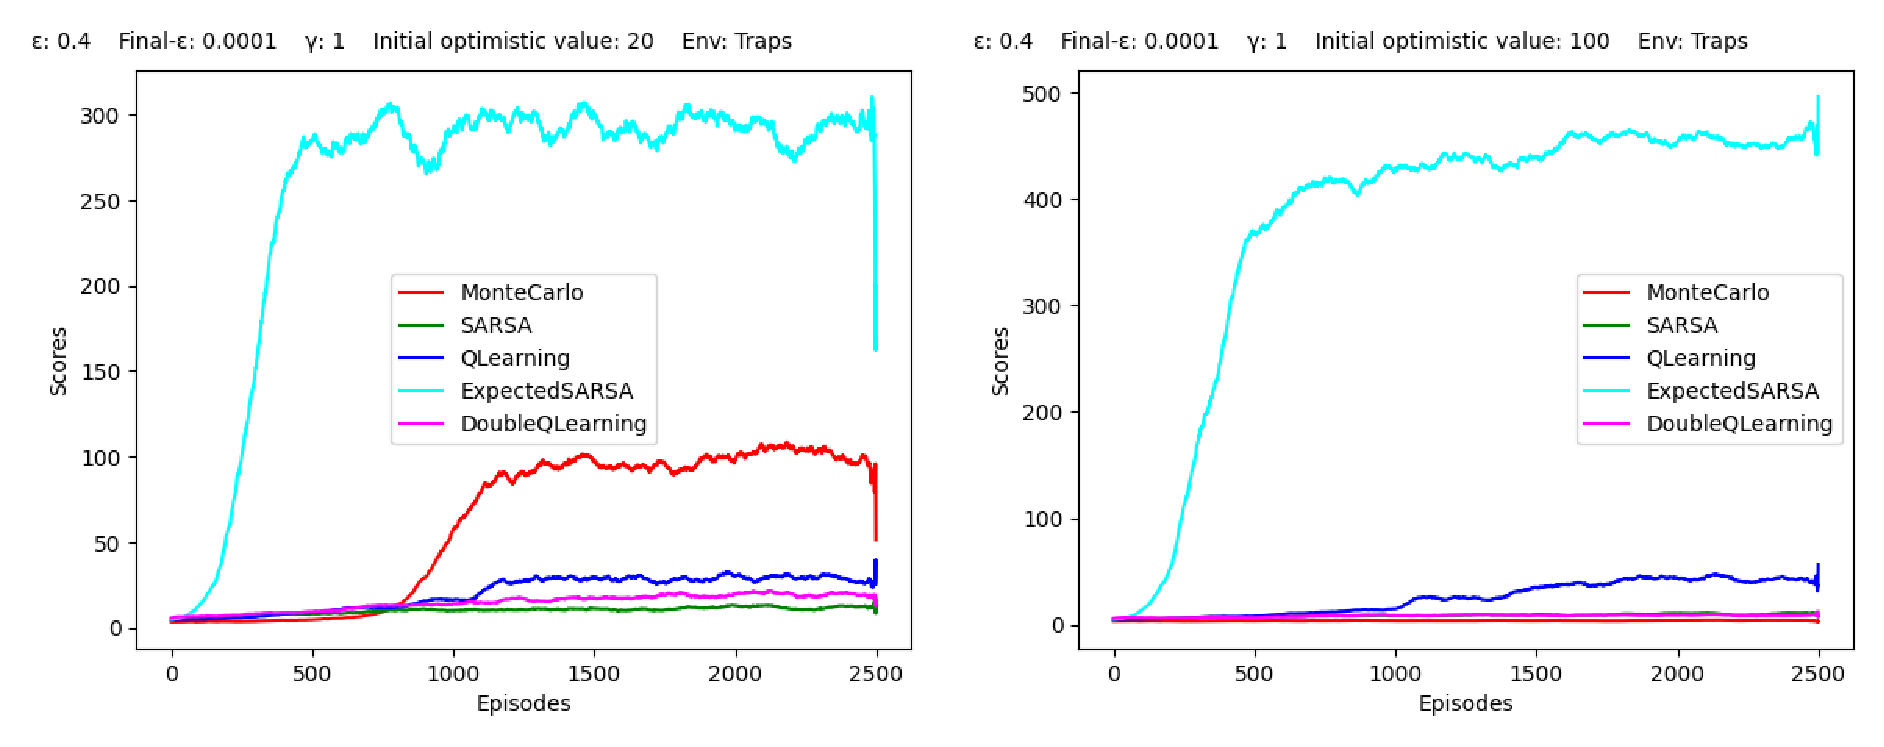
\includegraphics[width=\textwidth]{allTraps}
    \caption{All traps examples}
    \label{fig:alltraps_eg}
\end{figure}

This section delves into the exploration of a highly intricate environment of all traps combined, which is possibly the most complex one barring the full game. To clarify,\texttt{Traps} consist of all 10 individual traps mentioned in the previous section, and omit any bugs, virus or token type of obstacles. As depicted in Figure \ref{fig:alltraps_eg}, the majority of agents were unable to perform optimally in this environment. \texttt{ExpectedSARSA} was the only agent able to learn an optimal policy in any occurrence, as evidenced by its score nearing 500 in the right plot\footnote{It is worth mentioning that the plots for this environment have been smoothed with \texttt{window=100}.}, which was the approximate winning score value in all experiments. Moreover, \texttt{ExpectedSARSA} not only managed to learn an optimal policy once but did so with different hyperparameters and seed values on multiple occasions, leading to winning streaks of 30 games and early termination of the experiment. This outcome is the most favourable for any environment. The figure displays the averaged value of 9 seeds for all agents under the specified parameters. 

The experiments conducted for this environment were systematic and involved matching commonly used \texttt{eps} and \texttt{initOptVal} to test if the agents could learn. In these experiments, the difference in learning between the \texttt{ExpectedSARSA} agent and the others is even more pronounced. However, on the left plot visible in Figure \ref{fig:alltraps_eg}, and one instance, where \texttt{eps=0.4} and \texttt{initOptVal=20}, the \texttt{MonteCarlo} agent performed reasonably well, attaining an average score of approximately 100, which is substantially superior to the other agents, except for \texttt{ExpectedSARSA}.

\begin{figure}[h]
    \centering
    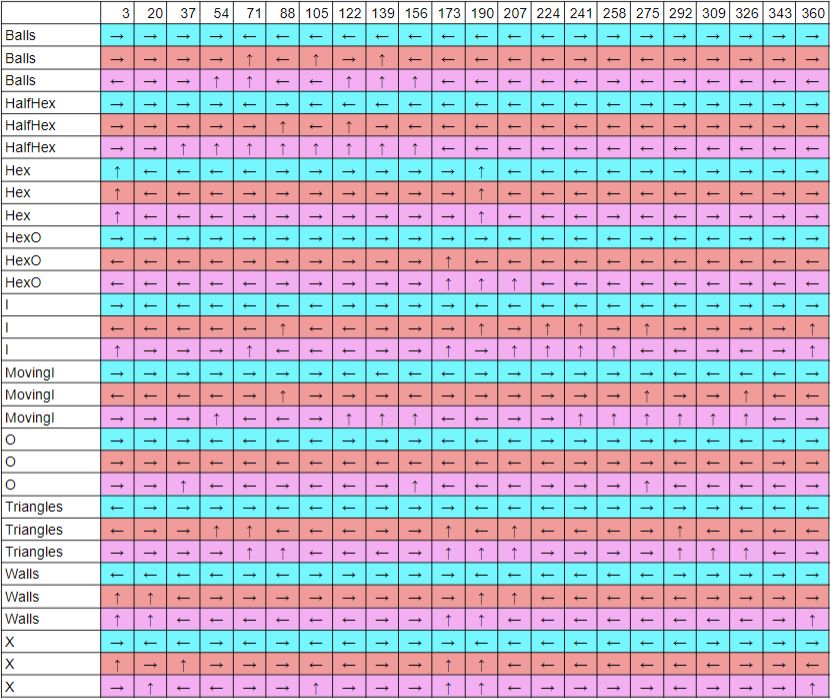
\includegraphics[width=0.8\textwidth]{allTraps_table}
    \caption{All traps with \texttt{ExpectedSARSA}, \texttt{MonteCarlo} and \texttt{DoubleQLearning} agents}
    \label{fig:traps_table_eg}
\end{figure}

When training in the all-traps environment I set the rots parameter to 22.  That's because it contains the Hex and Walls traps, which require a minimum of 22 rotations for learning to be feasible at all. This means that the number of states that with the individual trap environments corresponded to number of rotations, increased significantly. Considering that in this case we have 10 different trap types, there are 220 states with \texttt{Traps} environment. For that reason we picked \texttt{n=2500} for all of the experiments in this section. That's because in our experiments we've generally found that learning is most successful when the number of episodes is at least 10 times the number of states. Of course, it cannot be influenced by which states will be picked, since each game is generated randomly, but this was an estimation we used quite often during the experimentations. As a result of having this many \texttt{rots} values, with some simpler traps, there can be a lot of safe rotations that the agent can choose from. For that reason, going forward multiple adjacent states could be viable, if that particular trap requires for example \texttt{rots=6} when trained individually.

The content of the table in Figure \ref{fig:traps_table_eg} provides a comparison of policies from three different experiments, each reproduced with only one seed value, that yielded a satisfactory result. The purpose is to see how far off the agents were from an optimal policy. The blue rows represent the \texttt{ExpectedSARSA} agent, which performed with \texttt{eps=0.2} and \texttt{initOptVal=100}. The agent stopped an experiment early, after 437 games with initial number of games (\texttt{n}) being 2500. Considering it won 30 games in a row, each one lasting 15 levels, we can assume, with high probability, the learned policy is optimal for this environment. The red rows represent the \texttt{MonteCarlo} agent, which performed reasonably well with \texttt{eps=0.2} and \texttt{initOptVal=20}, winning 282/2500 games, but the experiment did not terminate early, suggesting a suboptimal policy. The pink rows represents the \texttt{QLearning} agent, which won 142/2500 games with \texttt{eps=0.4} and \texttt{initOptVal=20}. It should be noted that the combination of a seed value and hyperparameters that yielded the best results were picked for the \texttt{MonteCarlo} and \texttt{QLearning} agents, and in other cases, they won fewer or no games under this environment. Lastly it should be noted that, \texttt{SARSA(S)} and \texttt{DoubleQLearning}  performed poorly, with average scores in all experiments under all hyper parameter combinations, being not more than 20.

Multiple instances in the data show the phenomenon discussed in Section \ref{intbeh} of this chapter. For instance, upon closer examination of rotation values 54 and 71 in the rows pertaining to the Balls trap, it becomes evident that the \texttt{ExpectedSARSA} agent opted to alternate between those two rotation types, whereas the other two agents, \texttt{Monte Carlo} and \texttt{QLearning}, chose to proceed using only one or both of the rotations. This trend can be observed in several other cases within the data, and it is highly probable that, with so many rotation options available, any of the three methods would lead to the agent safely passing the trap. Nevertheless, it is a fact that \texttt{ExpectedSARSA} learned a better policy than \texttt{MonteCarlo} and \texttt{QLearning}. However, for certain traps, all or at least two of the agents had satisfactory policies (such as the \texttt{Hex} trap), whereas for others, \texttt{MonteCarlo} and/or \texttt{QLearning} were observed taking actions that could not be deemed optimal when compared to the \texttt{ExpectedSARSA} agent. An example of such an instance can be found in rotation values 275 and 292 with trap \texttt{X}, where the \texttt{QLearning} agent attempted to switch between the two rotations to pass, while both \texttt{ExpectedSARSA} and \texttt{MonteCarlo} avoided it, suggesting that remaining in that rotation was not safe and that the agent should try to move to another rotation in a timely manner.

\section{Tokens environment}
\begin{figure}[h]
    \centering
    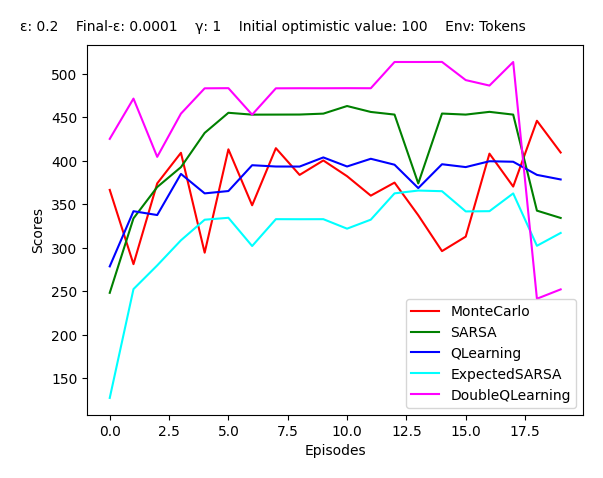
\includegraphics[width=0.6\textwidth]{tokensEnv}
    \caption{\texttt{Tokens} example}
    \label{fig:tokens}
\end{figure}

The Tokens environment is characterized by its simplicity, as it lacks obstacles that pose a lethal threat to the agent. The agent's task is to collect tokens at regular intervals to prevent its battery from draining completely. The number of rotations needed in this environment is six, making it relatively easy to train. Figure \ref{fig:tokens} illustrates that the average performance of all agents is commendable, even when \texttt{n=20}\footnote{Note that smoothing was applied to this plot.}. In subsequent sections, we will delve into more intriguing findings when tokens are incorporated into a larger environment, and explore their impact on the behaviour of the agents.

\section{Individual Bugs and Viruses environments}
\begin{figure}[h]
    \centering
    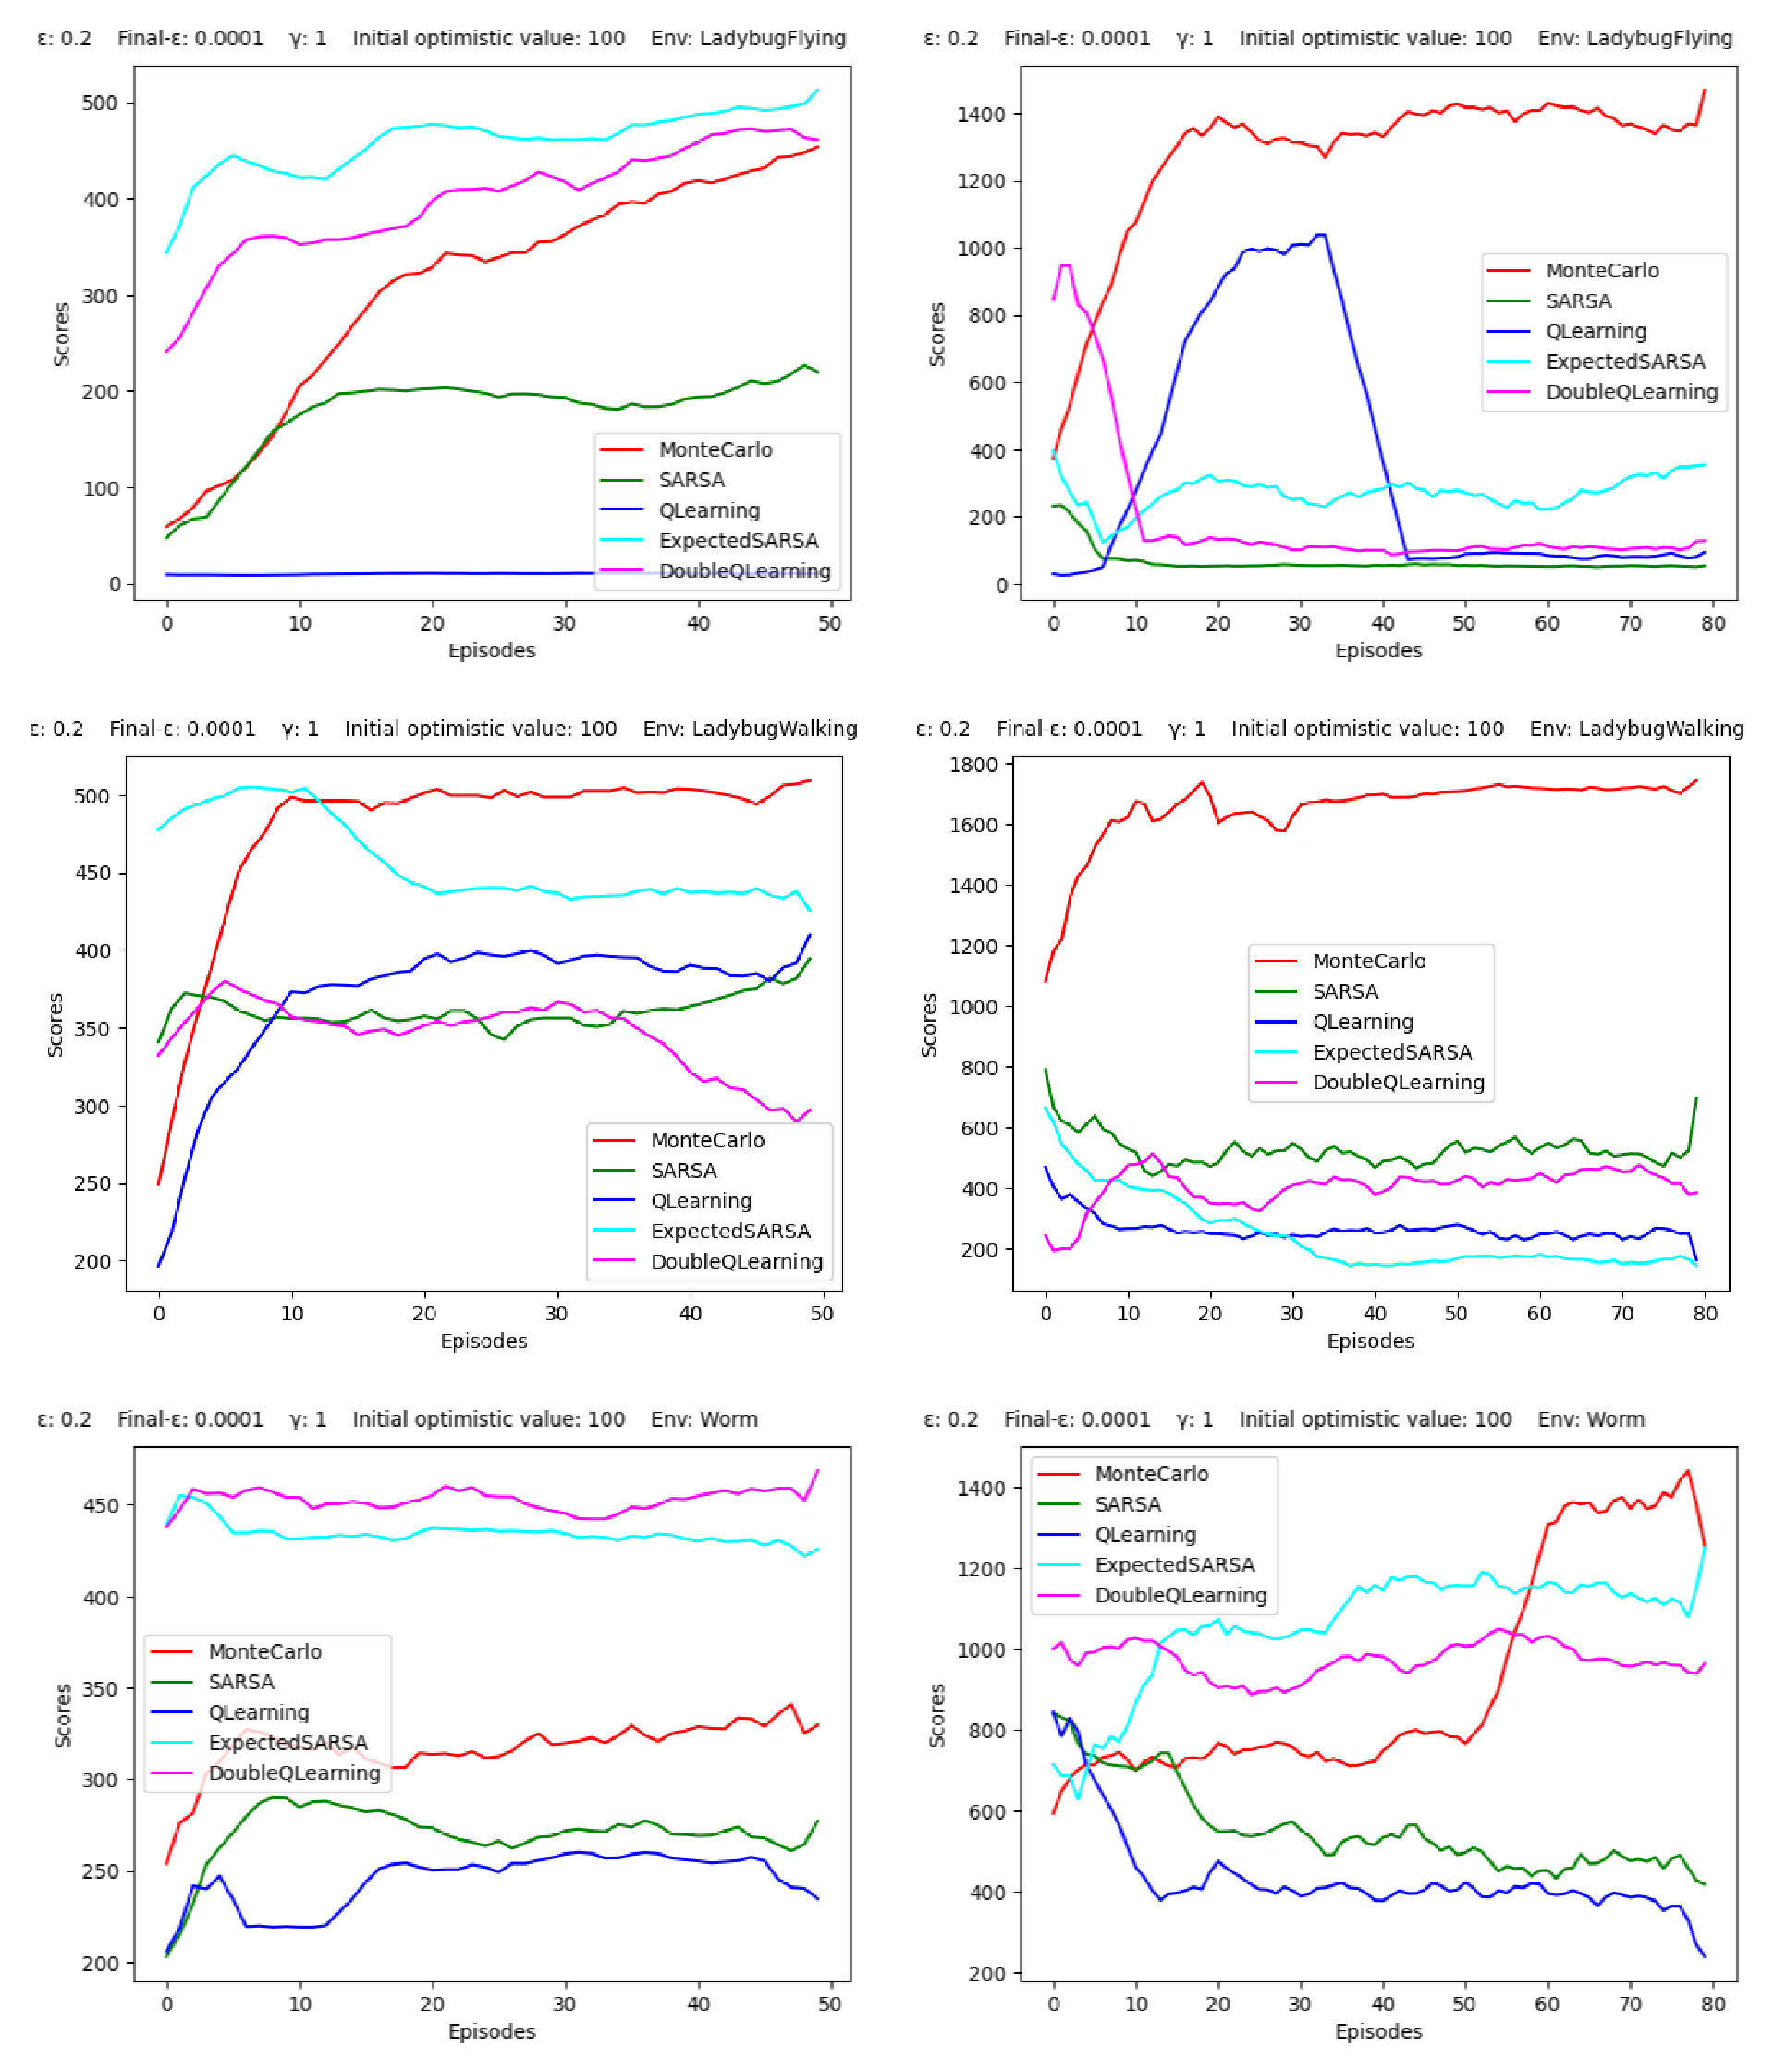
\includegraphics[width=0.9\textwidth]{bugs_ind}
    \caption{\texttt{LadybugFlying}, \texttt{LadybugWalking} and \texttt{Worm} environments examples}
    \label{fig:bugs_ind_eg}
\end{figure}

In this section, we aim to investigate two types of environments that have not been discussed before: Bugs and Viruses. These environments include three (\texttt{Worm, LadibugWalkingm LadybugFlying}) and two (\texttt{Bacteriophage, Rotavirus}) obstacles, respectively, and are different from environments that consist solely of trap-type obstacles. One key difference is that the agent can also use its ability to shoot in \texttt{Bugs} and \texttt{Viruses} environments. This means that, for the first time in this chapter, our agents have 6 actions to choose from, and we aim to analyse how this affects their behaviour.

We begin by showcasing the performance of all agents on individual bugs or viruses. For this purpose, we have evaluated their performance on 50 games, each with \texttt{eps=0.2} and \texttt{initialOptVal=100.0}. We chose these parameters as they resulted in the best overall performance of the agents. The plots presenting all agents in this section are an average of five different seeds, and each plot has been smoothed with a \texttt{window=10}. The left-hand side of both figures displays the agents' performance when shooting was not enabled, whereas the right-hand side depicts the scores when the agents could shoot.

\begin{figure}[h]
    \centering
    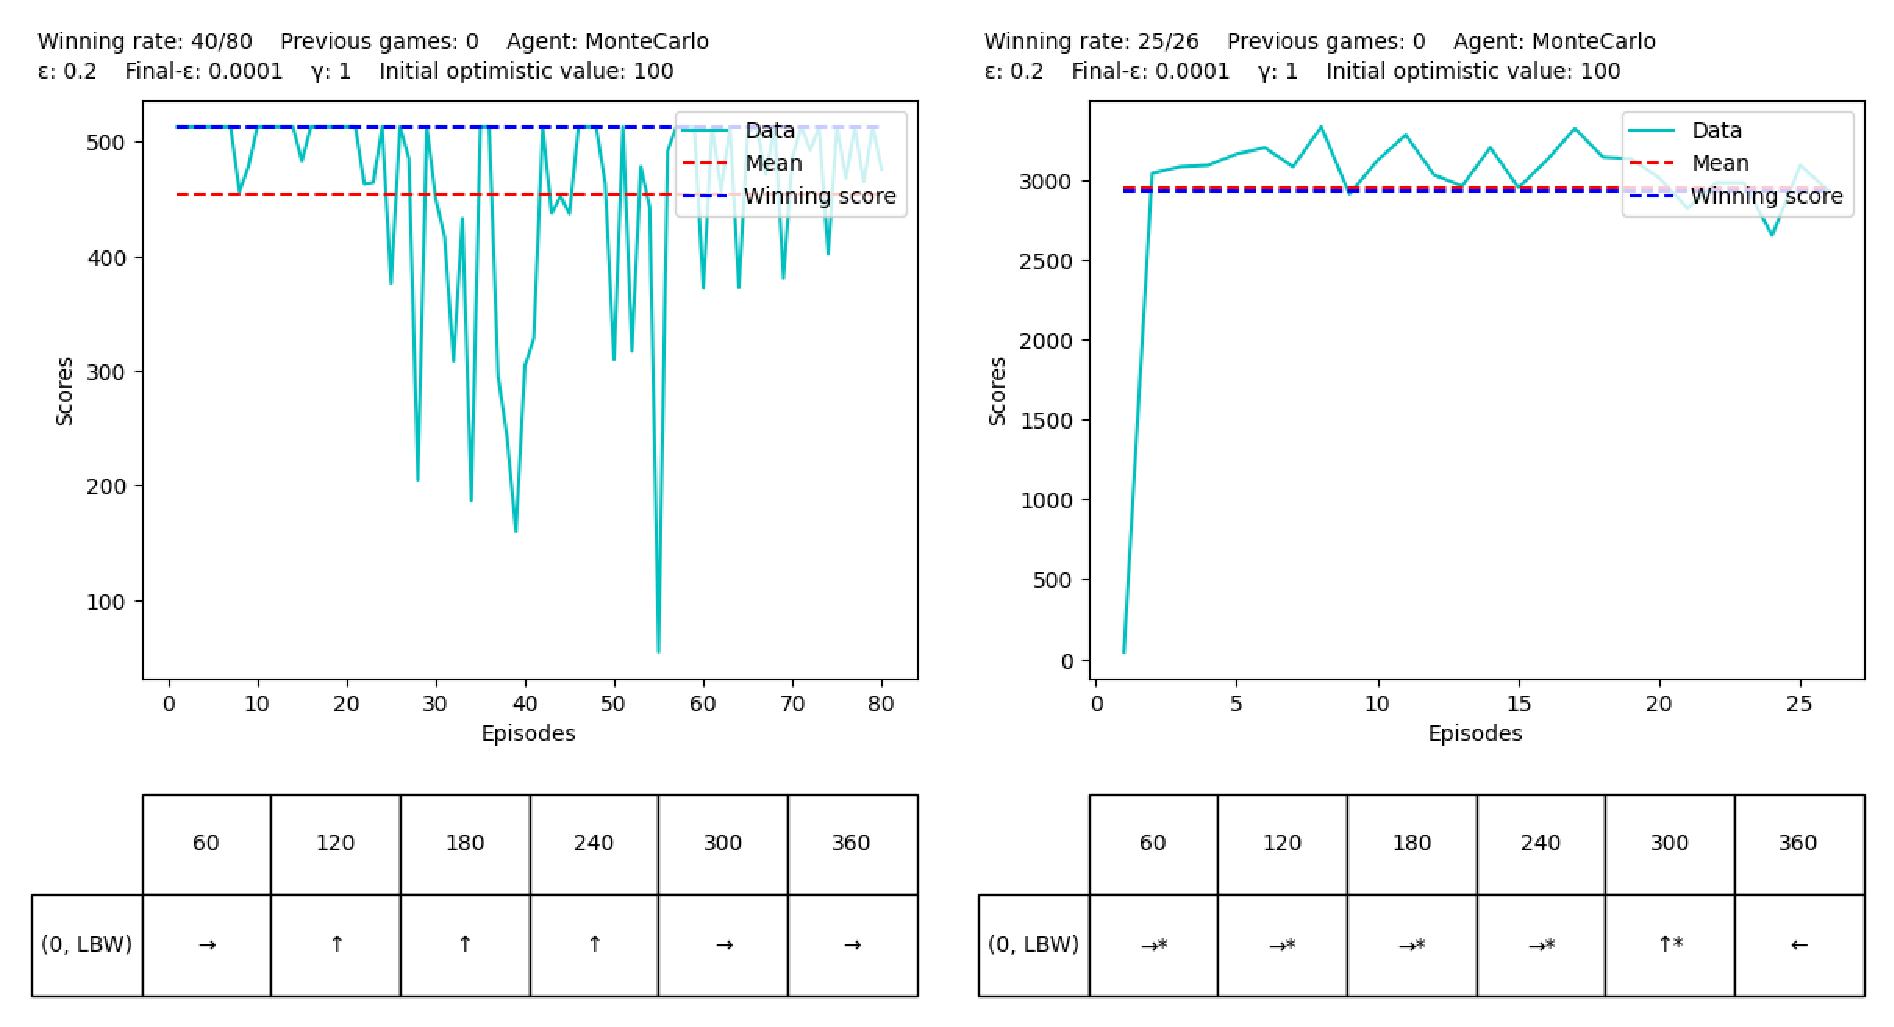
\includegraphics[width=0.8\textwidth]{bugs_ind_mc}
    \caption{\texttt{LadybugWalking} with \texttt{MonteCarlo} agent examples}
    \label{fig:bugs_ind_mc_eg}
\end{figure}

The category of obstacles referred to as bugs in the game environment behaves differently from viruses or traps. This is due to the fact that Hans, only loses energy upon contact with any of the bug type obstacles, and only when the battery life is depleted to 0\% does the game terminate, or when the game is won. The performance of some agents in this environment is lower than in others, as illustrated in Figure \ref{fig:bugs_ind_eg}. However, the \texttt{MonteCarlo} agent consistently performs well, particularly with the \texttt{LadybugWalking} obstacle. Conversely, the \texttt{QLearning} agent appears to perform poorly in this environment, suggesting that it may not be the most suitable method for these seemingly inconsistent bug obstacles. As battery life is not part of the state value, the ideal behaviour for the agent would be to either always shoot (if permitted) or always avoid the these obstacles. This behaviour is precisely what is observed in Figure \ref{fig:bugs_ind_mc_eg}, where the \texttt{MonteCarlo} agent does not shoot at all in the left plot (suggesting that its avoiding the obstacles), while in the right one, it shoots in almost all actions. Although the left plot may not have achieved an optimal policy, it has derived one that allows the agent to win at least 50\% of the time.

\begin{figure}[h]
    \centering
    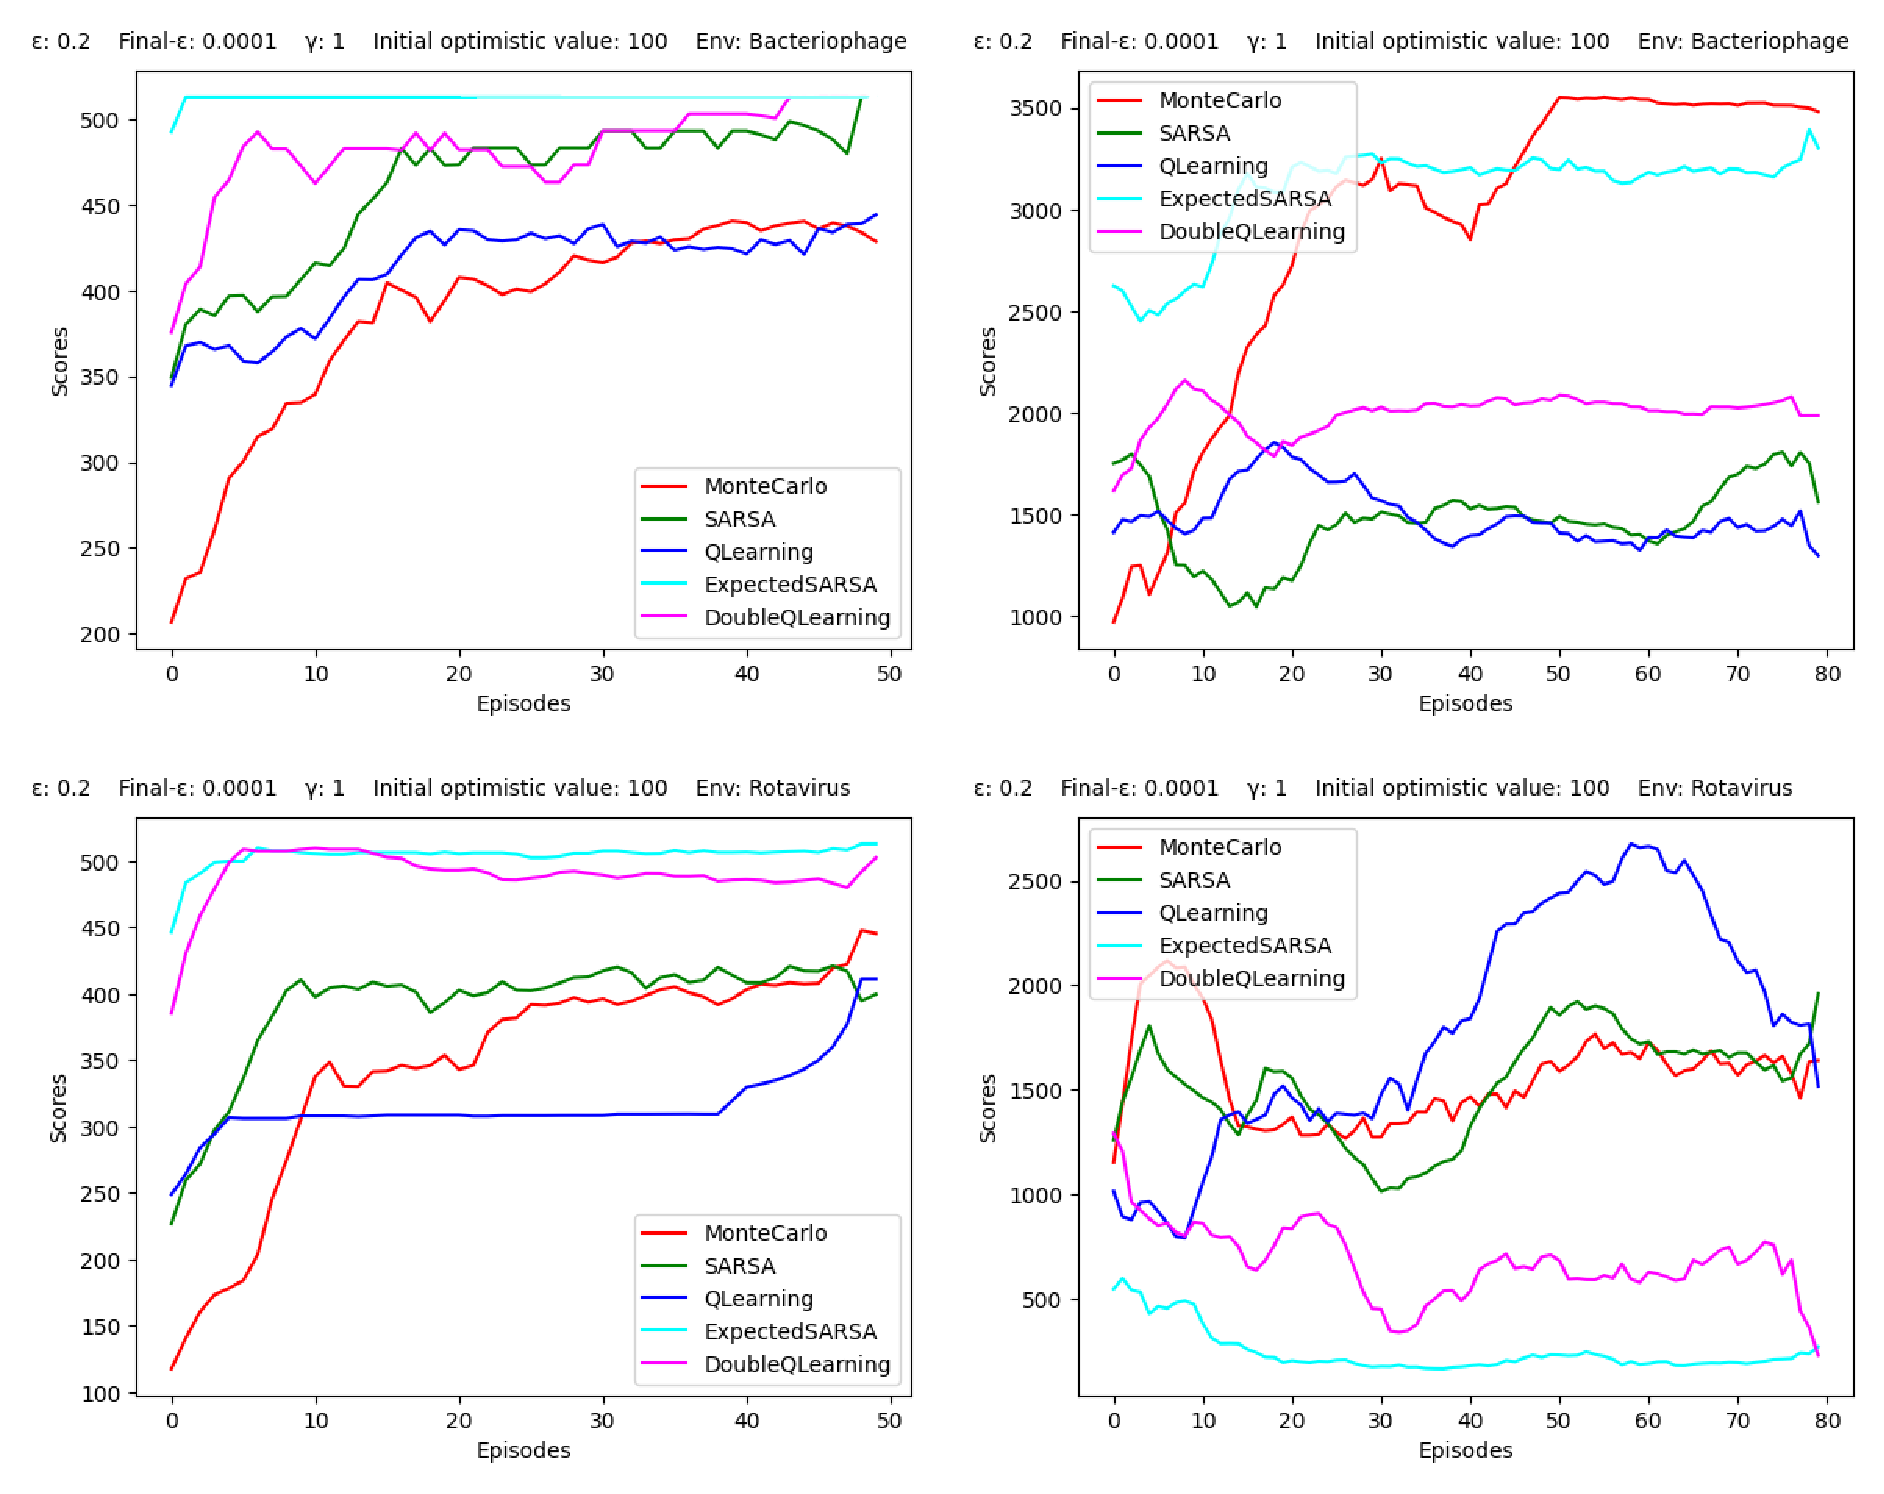
\includegraphics[width=0.8\textwidth]{viruses_ind}
    \caption{\texttt{Bacteriophage} and \texttt{Rotavirus} environments examples}
    \label{fig:viruses_ind_eg}
\end{figure}

Figure \ref{fig:viruses_ind_eg} displays the performance of the agents for each virus type obstacle. Notably, \texttt{ExpectedSARSA} exhibited a high level of performance in both cases where shooting was not enabled. However, in the case of \texttt{Rotavirus} when the shooting was involved, it performed the worst out of all the agents. It is possible that the agent was confused by the\texttt{Rotavirus} behaviour, since when Hans hits a \texttt{Rotavirus} for the first time, he becomes sick, and if it is hit again during his sick period, it results in his death. In contrast, the behaviour of \texttt{Bacteriophage} is more akin to the traps, as it kills Hans on the spot upon contact.

\begin{figure}[h]
    \centering
    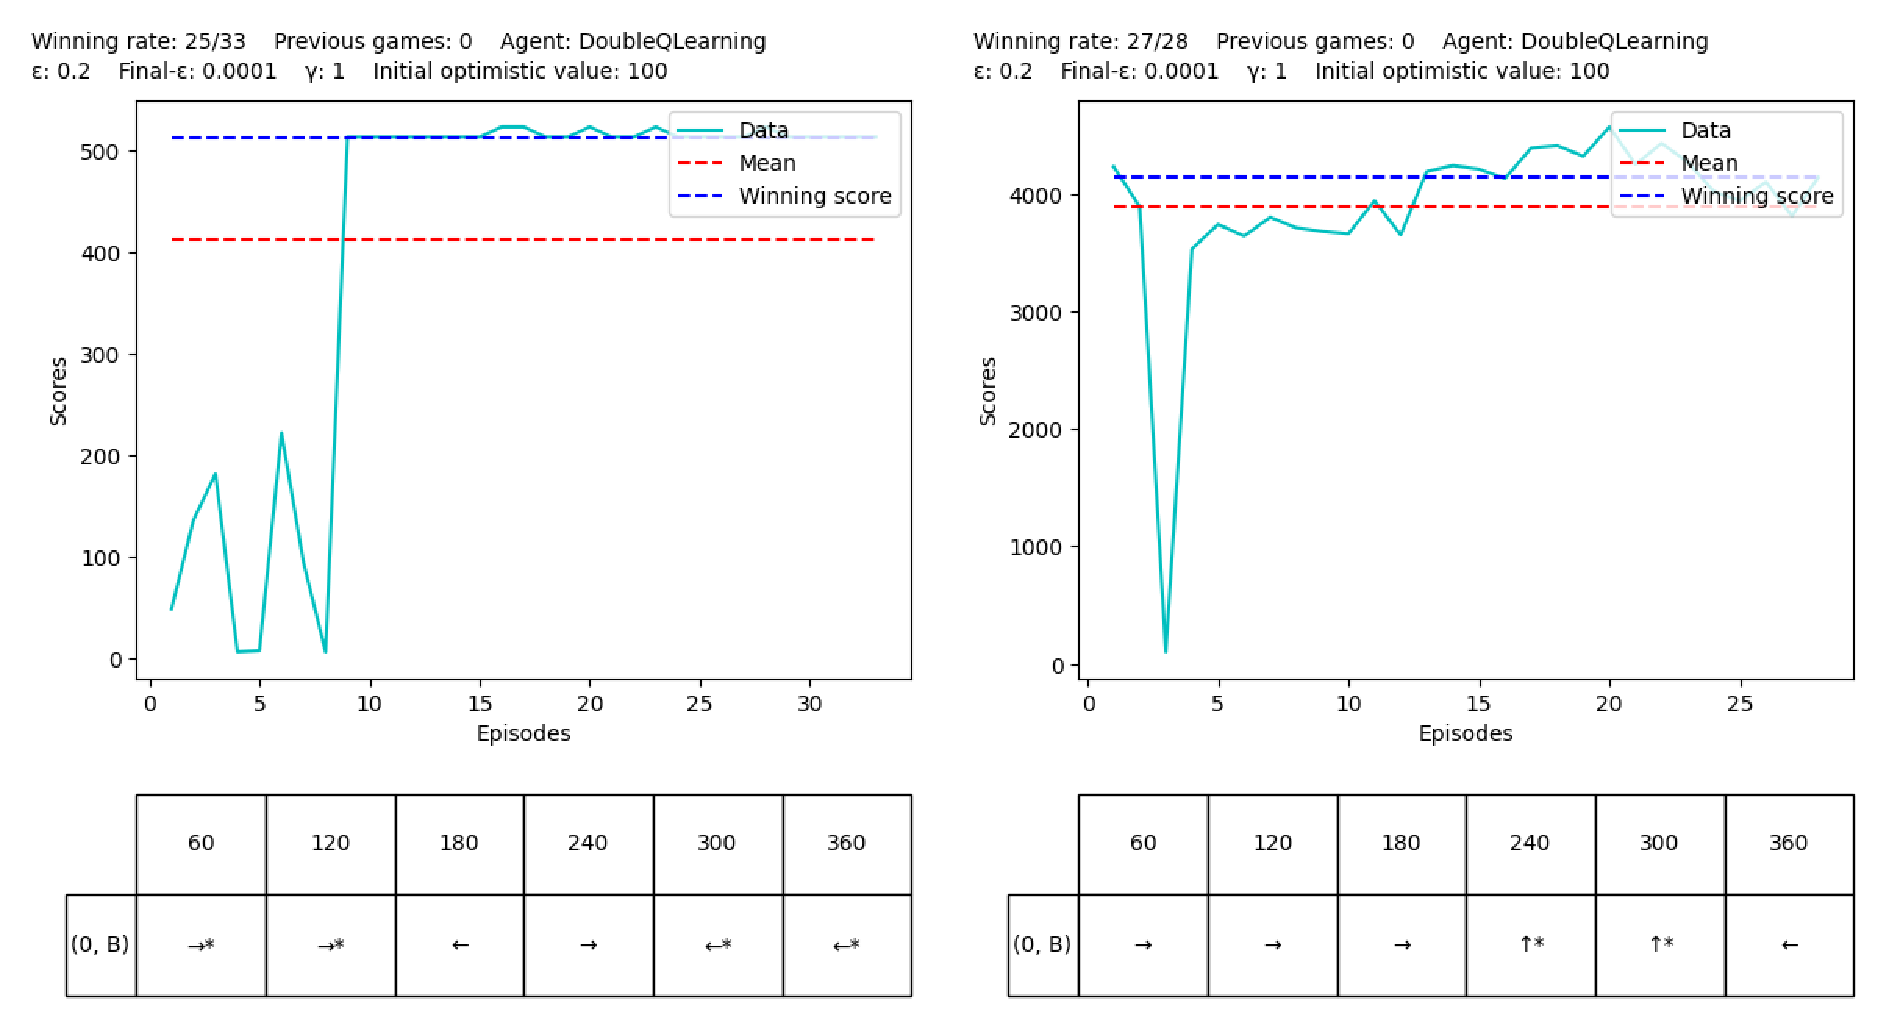
\includegraphics[width=0.8\textwidth]{viruses_ind_dql}
    \caption{\texttt{Rotavirus} environment with \texttt{DoubleQLearning} agent examples}
    \label{fig:viruses_ind_dql_eg}
\end{figure}

To diverge a little from the performance of the agents all together, lets take a look into Figure \ref{fig:viruses_ind_dql_eg} which shows two instances of the \texttt{DoubleQLearning} agent with the \texttt{Rotavirus} obstacle and \texttt{shooting=enabled}. Each plot used only one seed value and the smoothing was not applied. In both of the cases in this figure, the agent learned an optimal policy and thus terminated the game early. However, for the left plot, even though there are some actions in which the agent chooses to shoot, it doesn't actually shoot down any obstacles. This is evident by the fact that the winning score is only around 500, which is the minimum winning score achieved after 15 levels.  This might explain why in these conditions, the \texttt{DoubleQLearning} agent did not perform as well as some of the others in the overall performance analysis (Figure \ref{fig:viruses_ind_eg}). On the other hand, the right plot shows a policy in which that the agent learned to shoot down the \texttt{Rotavirus} obstacles and achieved a much higher winning score, demonstrating the importance of properly utilizing the shooting action when it is enabled.

\section{Bugs and Viruses environments}
\begin{figure}[h]
    \centering
    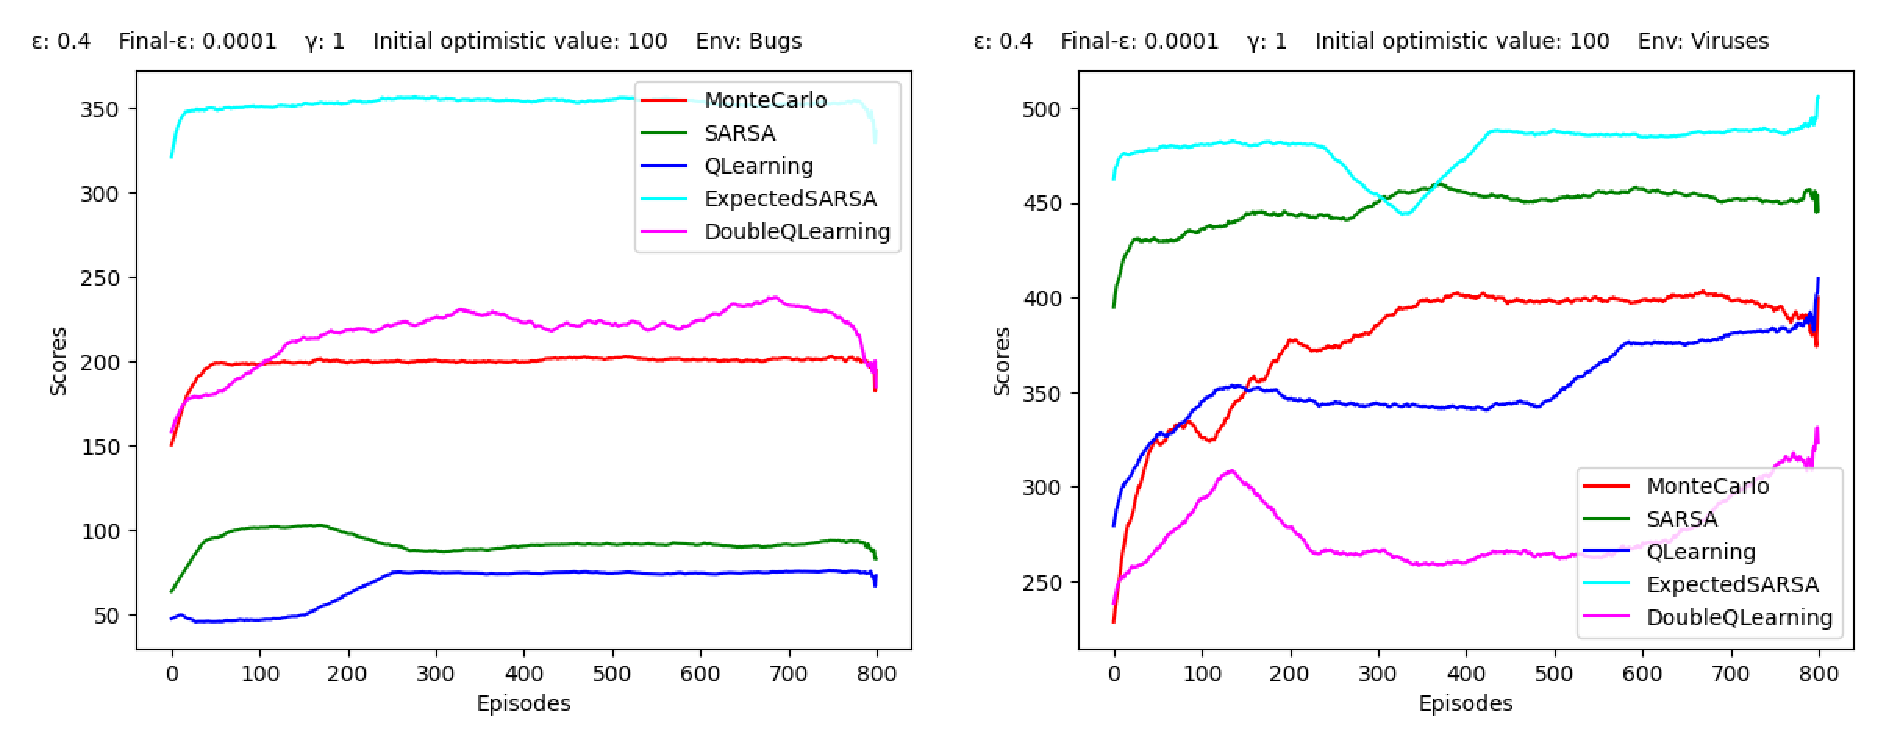
\includegraphics[width=0.9\textwidth]{BV800ns}
    \caption{\texttt{Bugs} and \texttt{Viruses} environments examples}
    \label{fig:bv800ns_eg}
\end{figure}

The current section compares the performance of agents in the full \texttt{Bugs} or \texttt{Viruses} environments and their combination with \texttt{Tokens} when faced with the same hyperparameters. Plots that display the performance of all agents in this section are averaged over 10 seeds and smoothed with \texttt{window=100}. In Figure \ref{fig:bv800ns_eg} we see the average performance of the agents when shooting is not allowed. Similar to the traps environment, the \texttt{ExpectedSARSA} agent exhibited the best performance. On the other hand, when faced with the full \texttt{Bugs} environment, \texttt{QLearning} agent showed similar behaviour to that seen on individual bugs obstacles and performed worse than the other agents.

\begin{figure}[h]
    \centering
    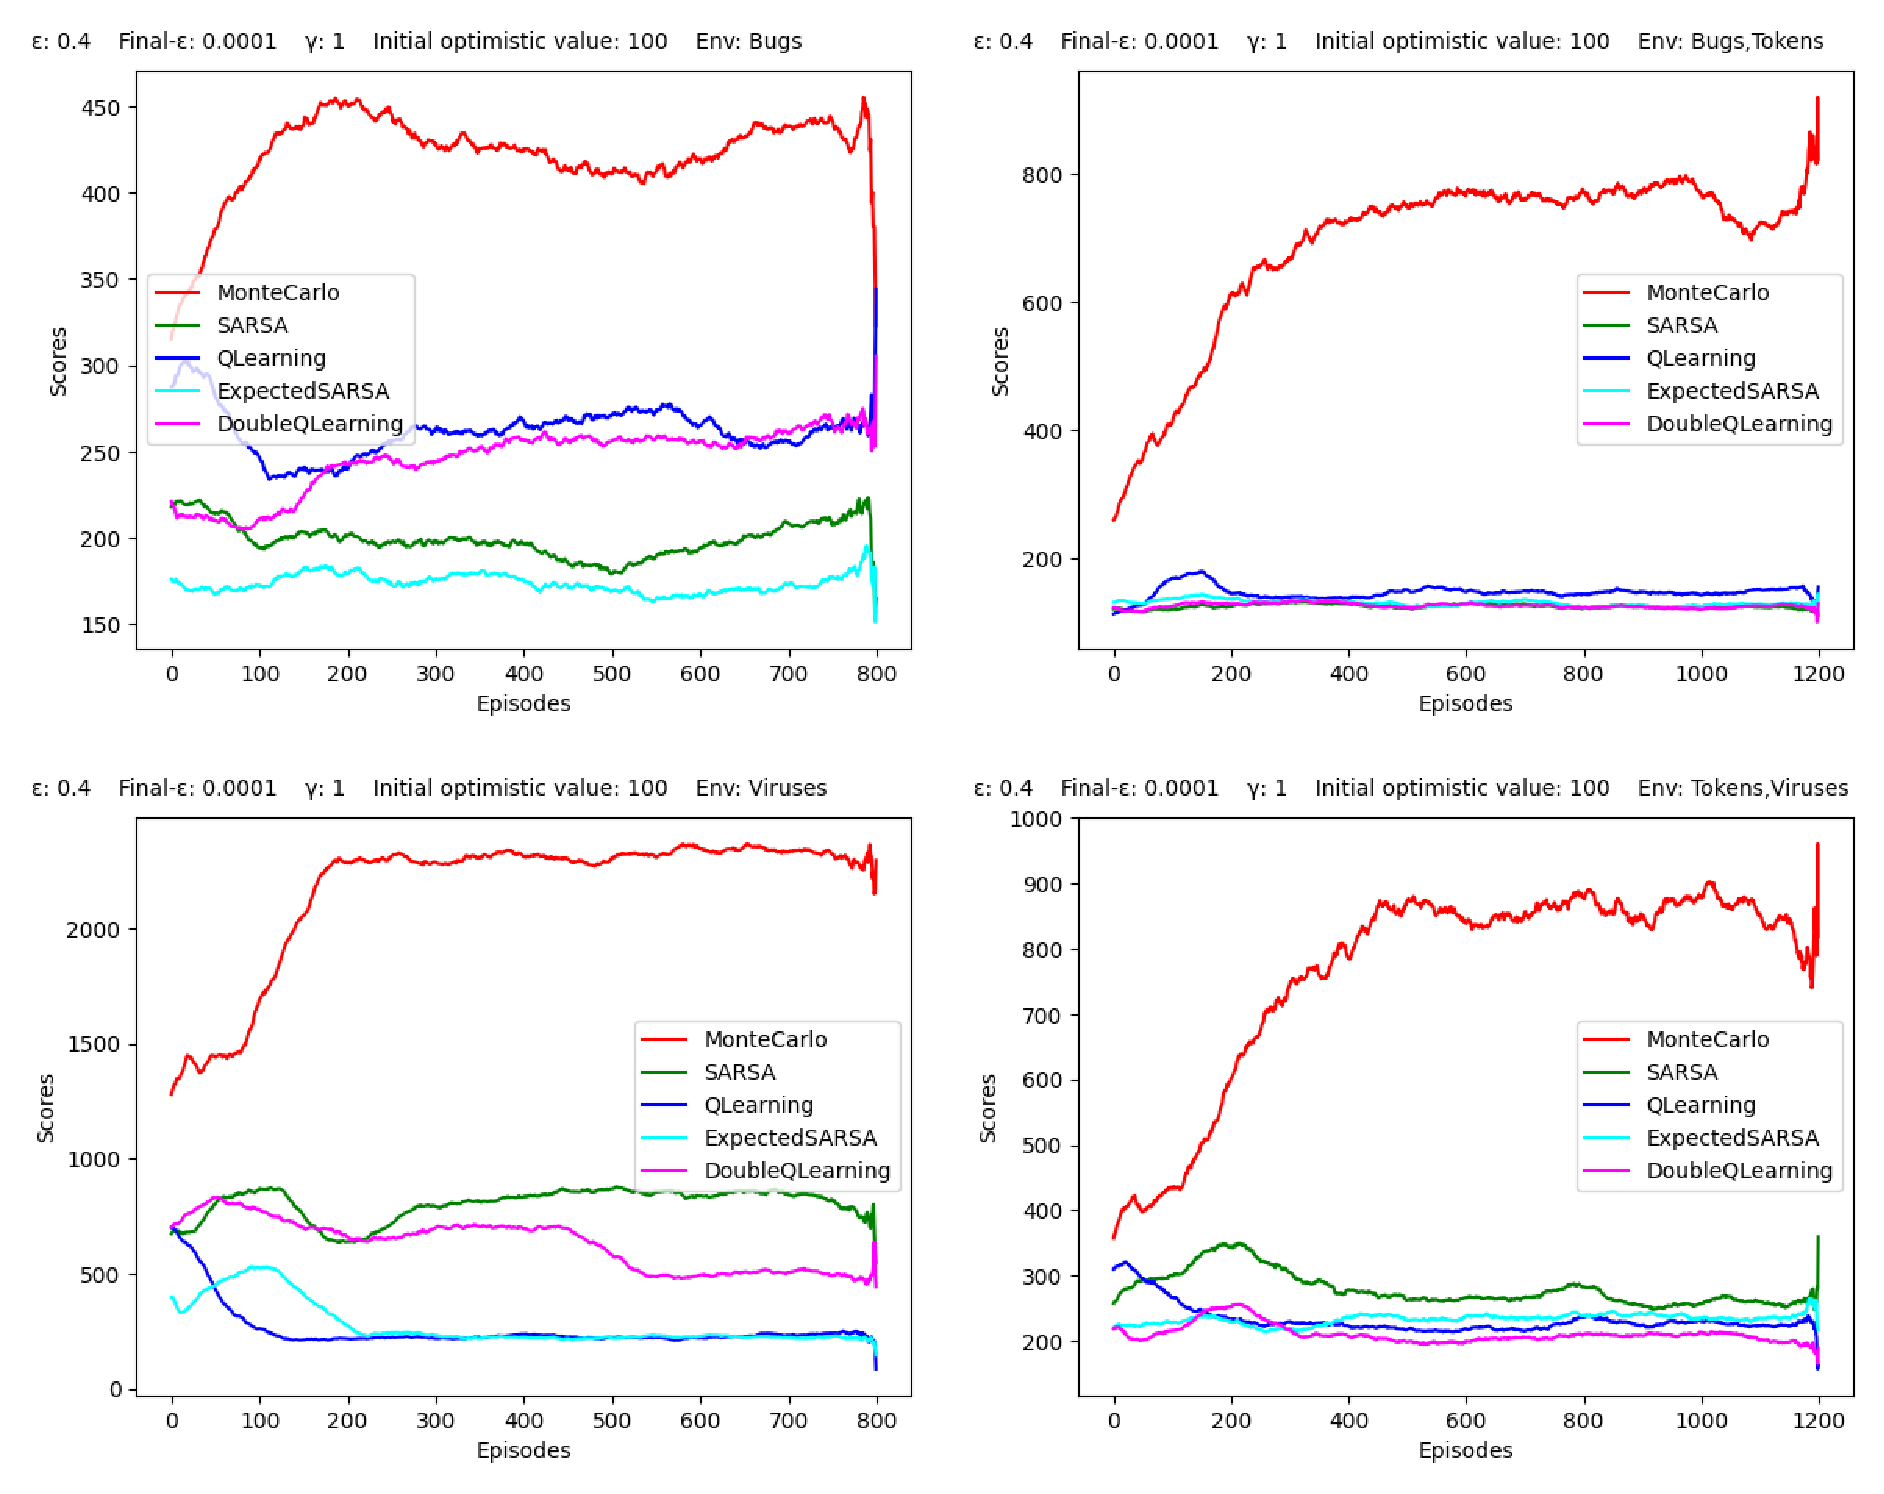
\includegraphics[width=0.8\textwidth]{bbt_vvt}
    \caption{\texttt{Bugs},\texttt{Viruses} and their combination with \texttt{Tokens} examples}
    \label{fig:bbt_vvt_eg}
\end{figure}

Figure \ref{fig:bbt_vvt_eg} shows plots where shooting actions are available to the agent. Here, the \texttt{MonteCarlo} agent had the best performance in all four cases. An interesting result is that when faced with \texttt{env=[Bugs,Tokens]}, this agent performed better than in the only \texttt{Bugs} environment, while with \texttt{env=[Viruses,Tokens]}, it performed worse than with \texttt{Viruses} alone. Considering how running into a bug influences Hans, adding \texttt{Tokens} to the \texttt{Bugs} environment was beneficial as long as the tokens were picked up when possible and the agent was conservative with shooting. In contrast, in the environment containing both \texttt{Viruses} and \texttt{Tokens}, the agent could still easily lose if Hans rans into \texttt{Bacteriophage} once or \texttt{Rotavirus} twice in a row. When having unlimited shooting in \texttt{Viruses} environment alone, all agents performed much better than when \texttt{Tokens} were part of it as well.

Overall, in environments that combine Tokens, the ratio of shooting and no shooting actions was approximately even. 

\begin{figure}[h]
    \centering
    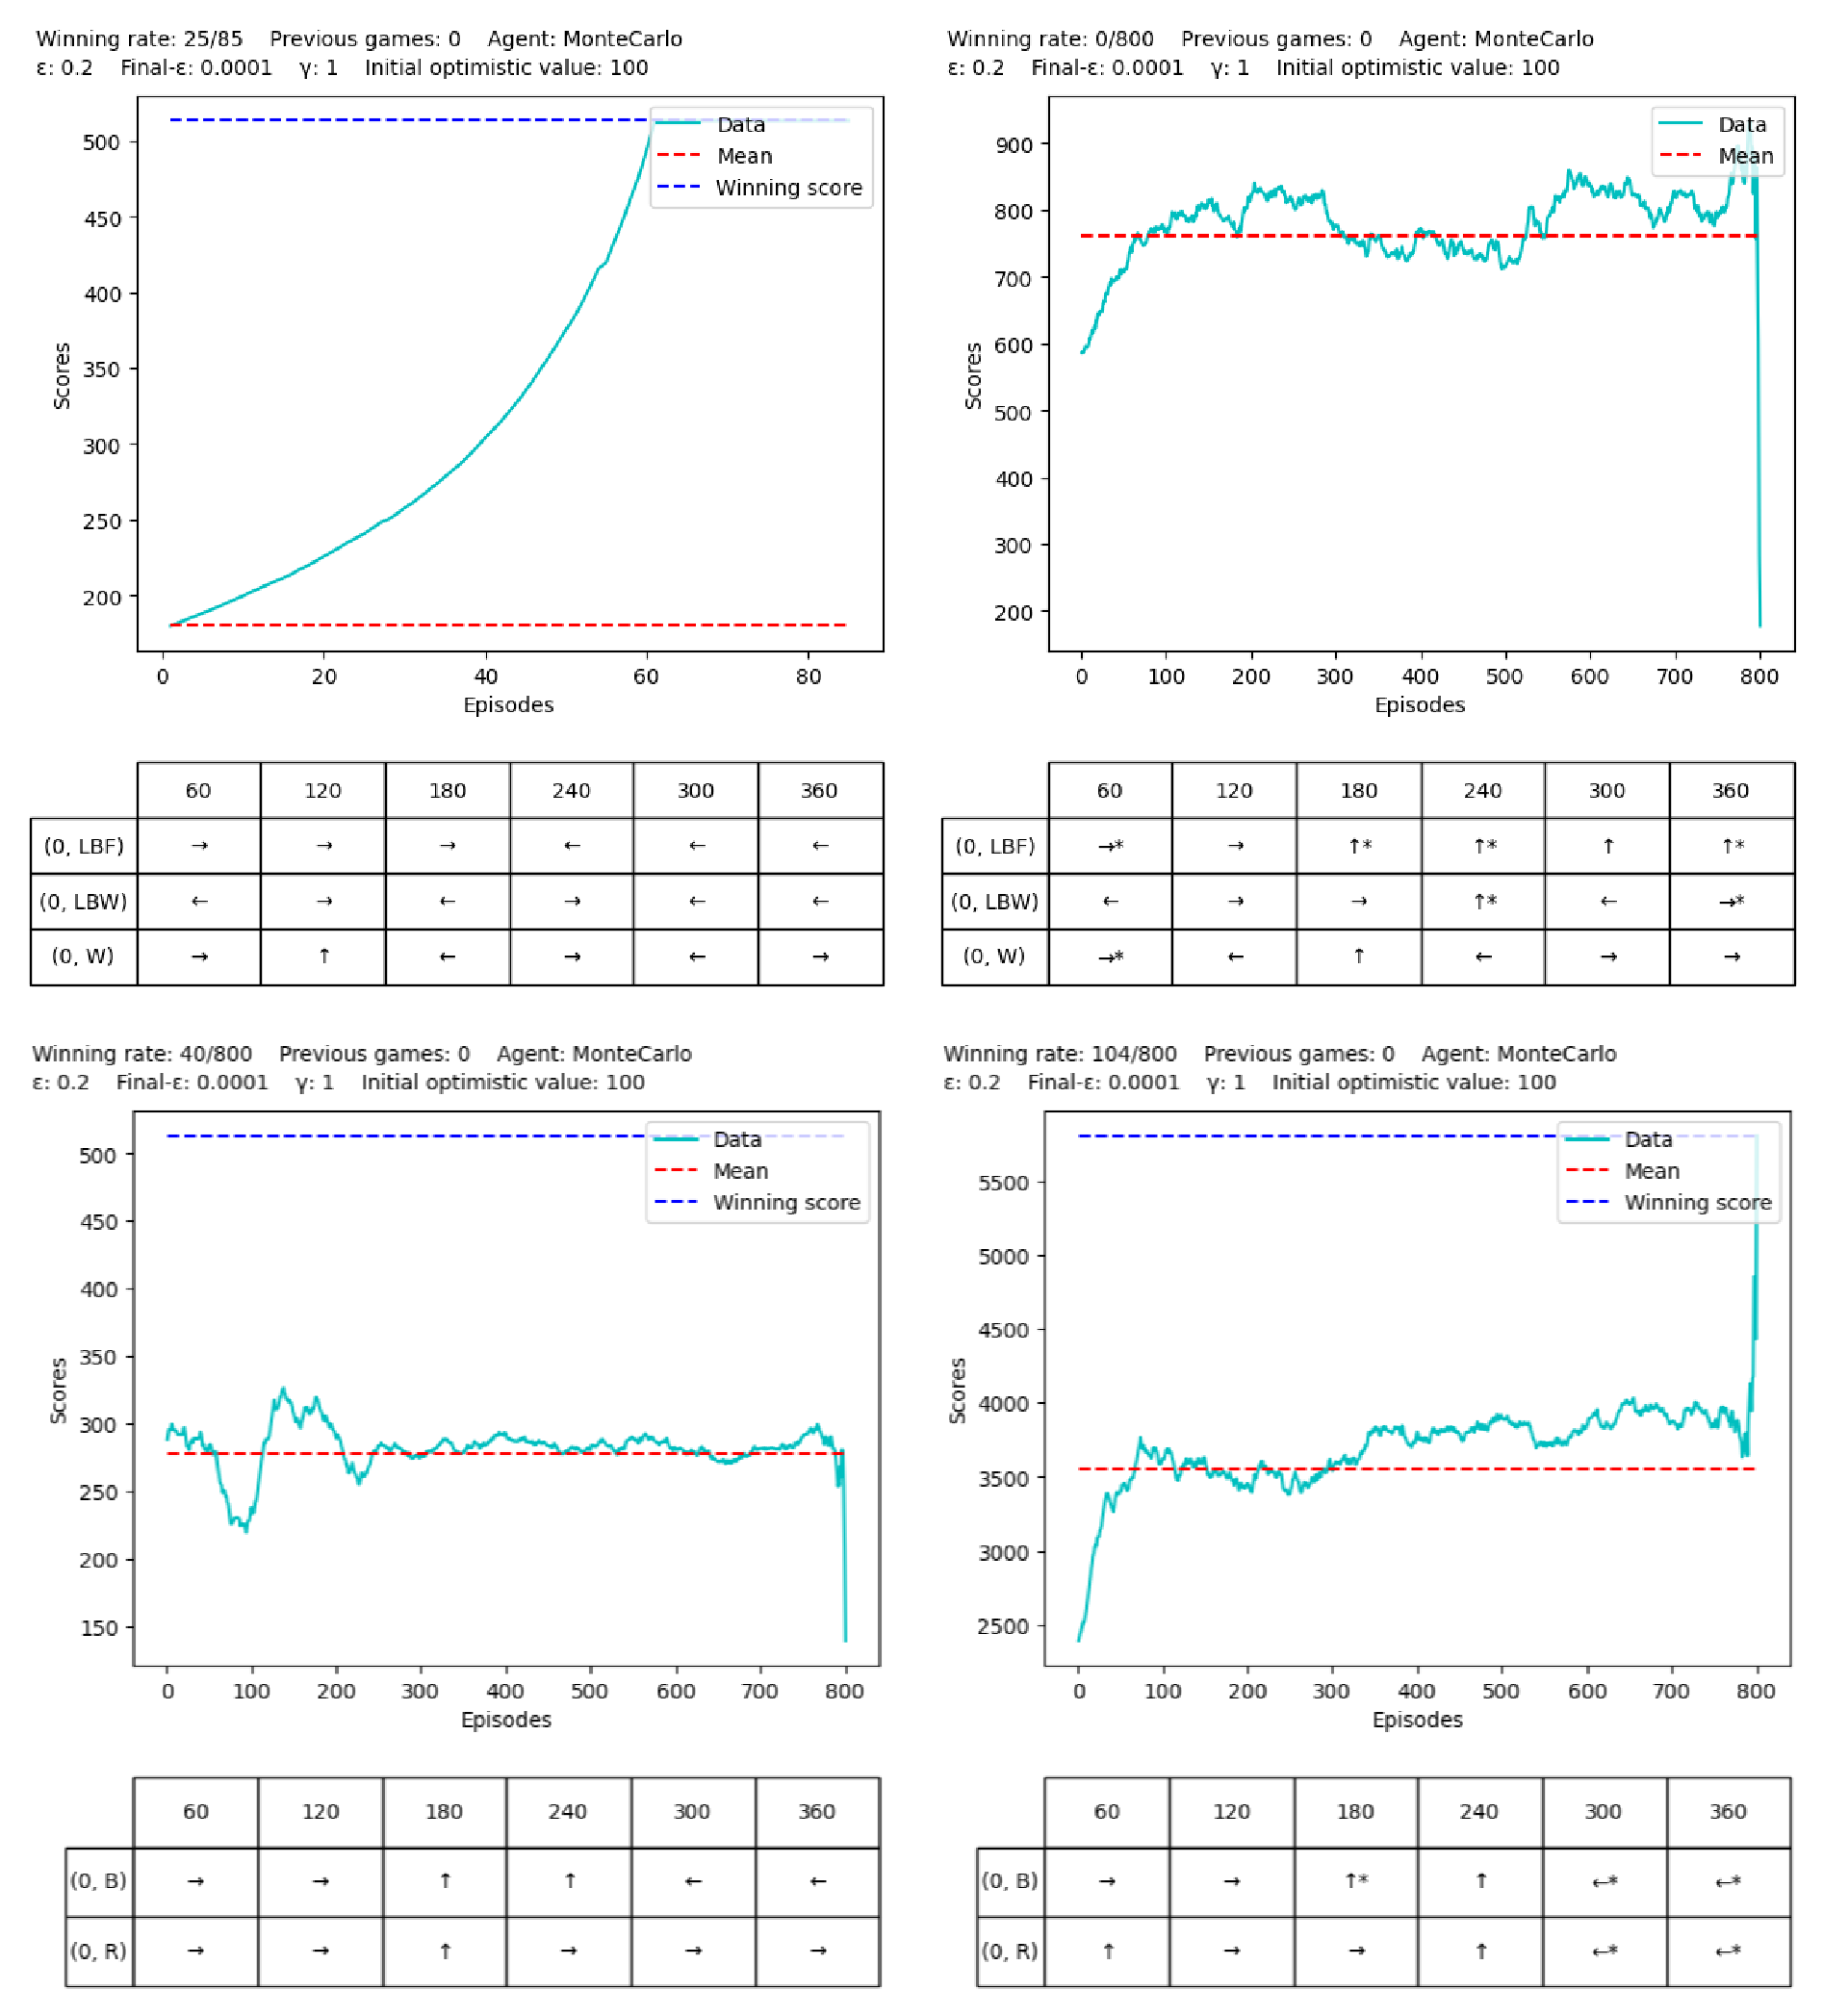
\includegraphics[width=\textwidth]{BV_02_100_1}
    \caption{\texttt{Bugs} and \texttt{Viruses} with and without shooting comparison}
    \label{fig:BV_02_100_1_eg}
\end{figure}


In Figure \ref{fig:BV_02_100_1_eg}, the performance of \texttt{MonteCarlo} agent shown environments is displayed for specific hyperparameters and with the same seed value (smoothing window value is 100). For each environment, two plots were created, one where the agent is allowed to shoot and another where shooting is disabled. The two plots depicting \texttt{Bugs} exhibit noticeable differences, as the agent found an optimal policy when shooting was not available. With shooting enabled, even though the direction of the agent's movement for each state is quite similar to the ones in the first plot, it failed to win any games. In contrast, with the \texttt{Viruses} environment, the agent's movement is almost identical in both cases, and the plot shows that the agent performed similarly well, with the right plot showing an average and winning scores approximately 10 times higher than on the left, as a consequence of the ability to shoot and due to that gain higher scores.

\section{Full game environment}
In this section, we explore the performance of the agents in the most challenging environment, full game. The results of these experiments are not surprising, given the complexity of the environment. In the figures presented in this section, we averaged the results of 10 seeds, and each plot was smoothed with a window of 100. The left side of the plots shows the performance of the agents in the environment where shooting is disabled, while the right side shows the environment where shooting is enabled. The right side was trained on 2000 more games than the left one considering that the number of actions possible increased.

\begin{figure}[h]
    \centering
    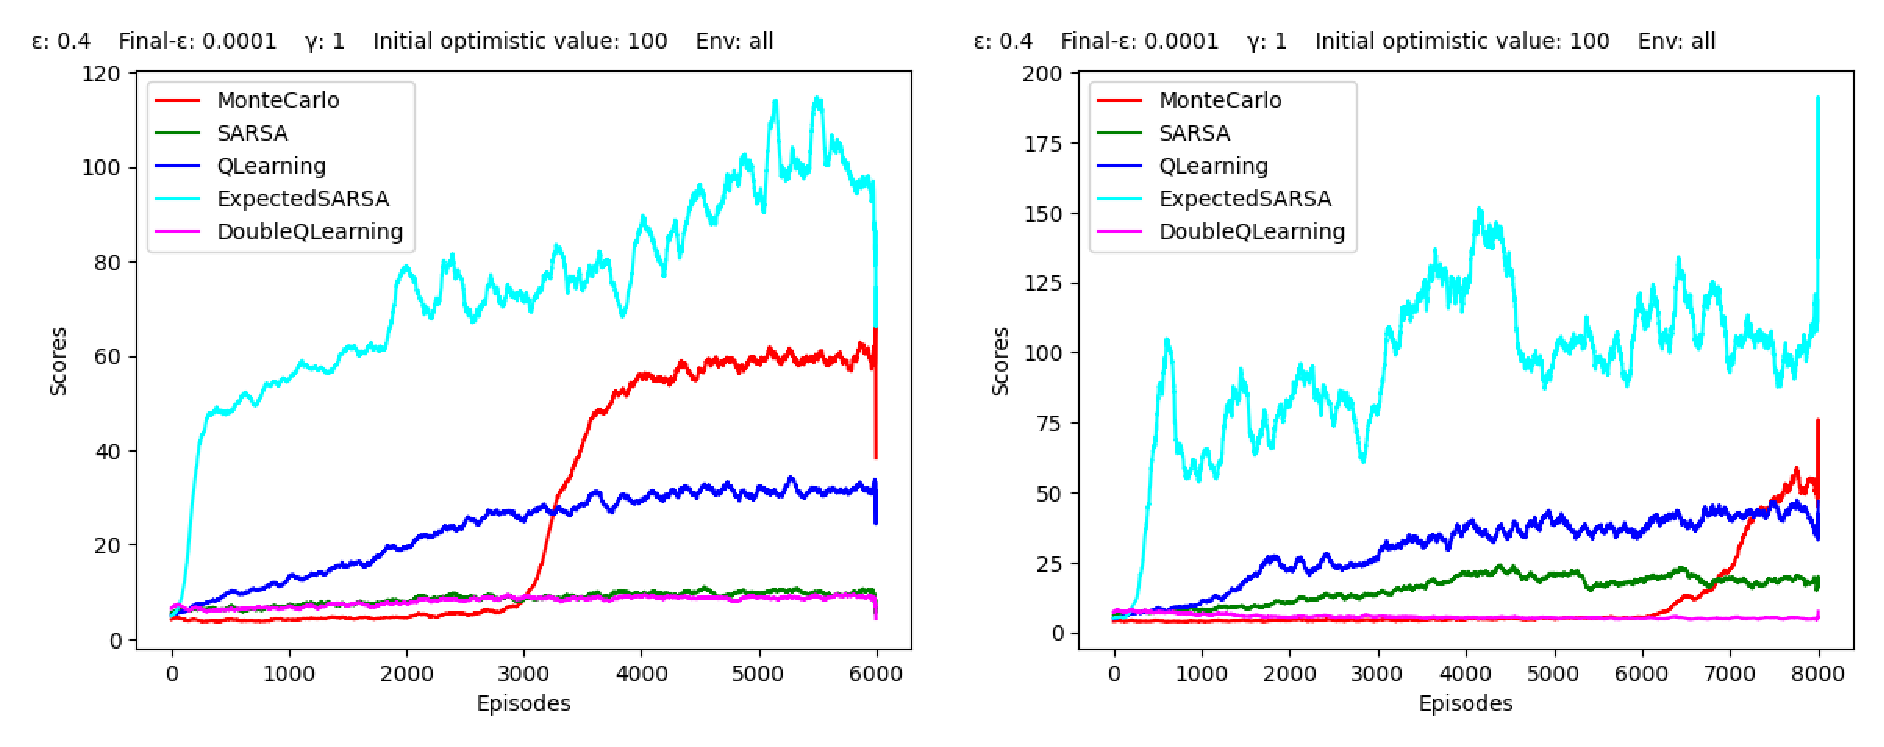
\includegraphics[width=0.8\textwidth]{full_game}
    \caption{Full game example}
    \label{fig:full_game_eg}
\end{figure}

Looking at Figure \ref{fig:full_game_eg}, we can see that in the environment without shooting, \texttt{ExpectedSARSA} performed the best, as expected. The scores of \texttt{MonteCarlo} and \texttt{QLearning} agents were not too bad, considering the complexity of the environment and the fact that \texttt{QLearning} agent underperformed in the \texttt{Bugs} environment. On the right plot, \texttt{ExpectedSARSA} is still in the lead compared to the other agents. However, considering that the agents were allowed to shoot in this case, the scores did not improve significantly.

\begin{figure}[h]
    \centering
    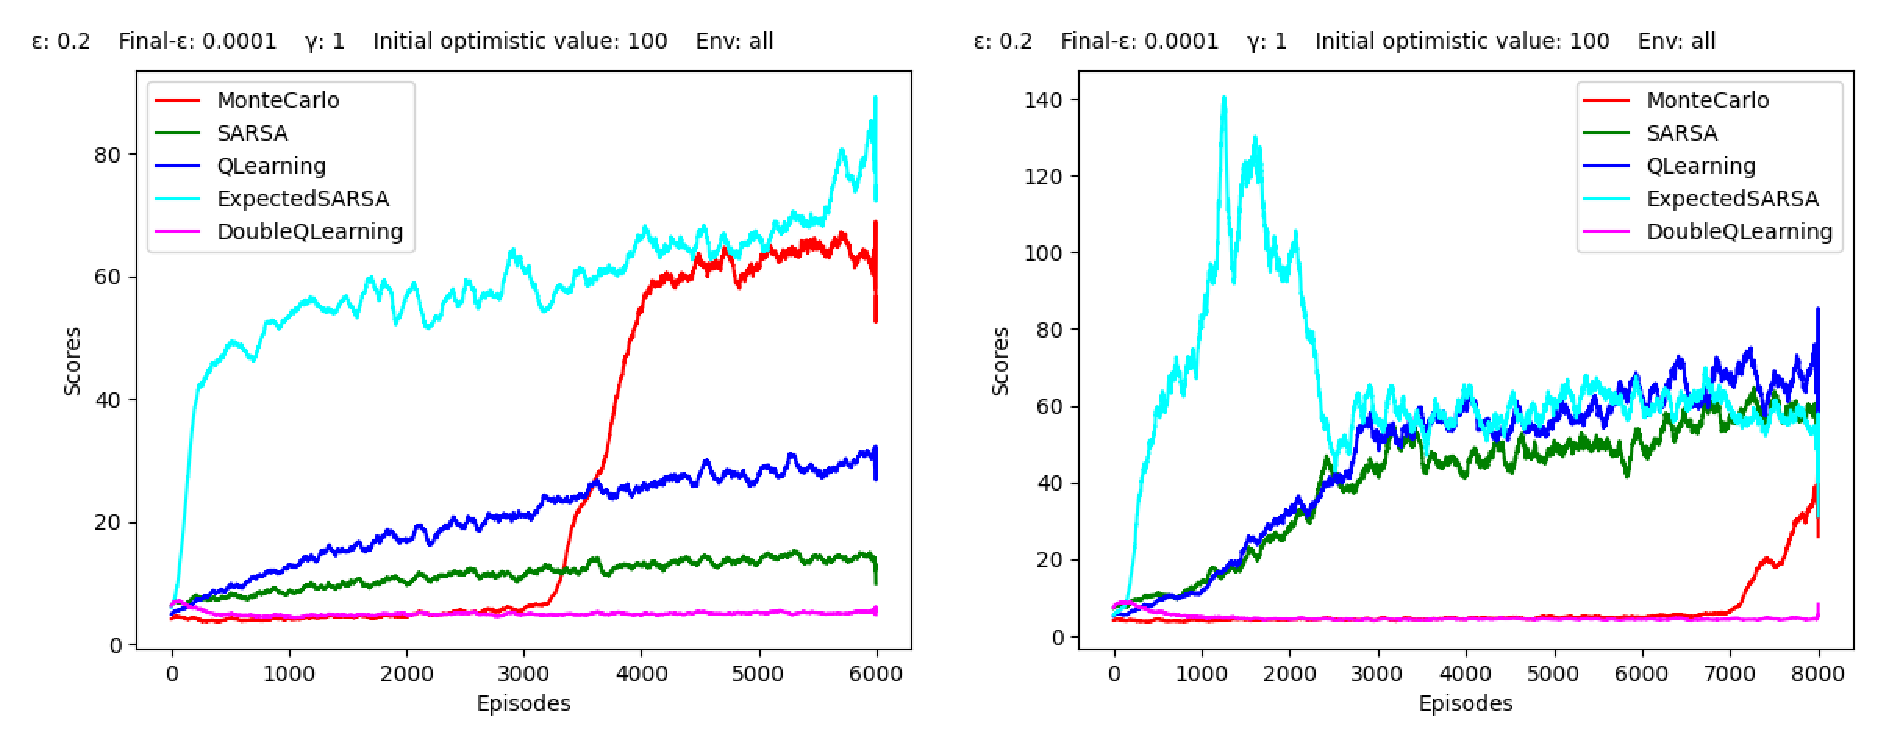
\includegraphics[width=0.8\textwidth]{full_game_cf}
    \caption{Catastrophic forgetting example}
    \label{fig:full_game_cf_eg}
\end{figure}

In Figure \ref{fig:full_game_cf_eg} we can observe an occurrence that has not been discussed before but is present throughout our experiments, namely the concept of catastrophic forgetting. As the name suggests, this is the notion that the agent learns a good policy and due to further exploration of the environment, the policy changes to something suboptimal. Ideally, the agent would come back to the previous policy, but more often than not, this is not the case. In the plot on the right, we can see that this is exactly what happened to the \texttt{ExpectedSARSA} agent during this experiment. The policy it learned in the first couple of thousand games was by far optimal, but it achieved a better score than the policies used after the sudden drop at approximately 2500 games.

\begin{figure}[h]
    \centering
    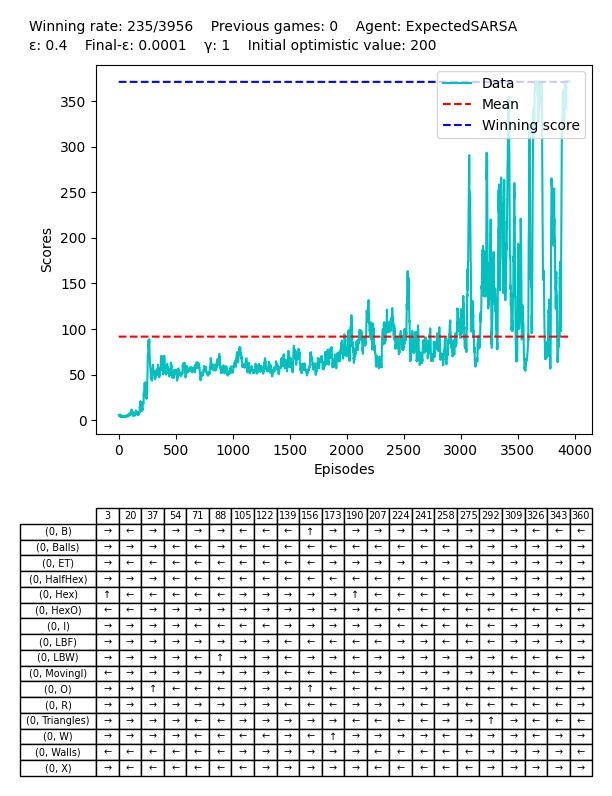
\includegraphics[width=0.7\textwidth]{full_game_es_win}
    \caption{Full game with \texttt{ExpectedSARSA} example}
    \label{fig:full_game_es_eg}
\end{figure}

The highly anticipated encounter detailed in Figure \ref{fig:full_game_es_eg} showcases a noteworthy outcome, as it portrays the \texttt{ExpectedSARSA} agent learning to play a full game by discovering an optimal policy under specific parameter settings and only one seed value. As part of the figure we can see the policy the agent acquired. This example serves as an illustration of how reinforcement learning agents are capable of learning to play this game when given the right conditions. However, it is important to note that this was a singular occurrence, and no similar outcomes were observed when shooting actions were introduced to the experiments. It is reasonable to conclude that while it may not be impossible for the agent to learn such a policy again, it may necessitate obtaining a fortuitous seed value.

\section{Interesting behaviours}
\label{intbeh}
\begin{figure}[h]
    \centering
    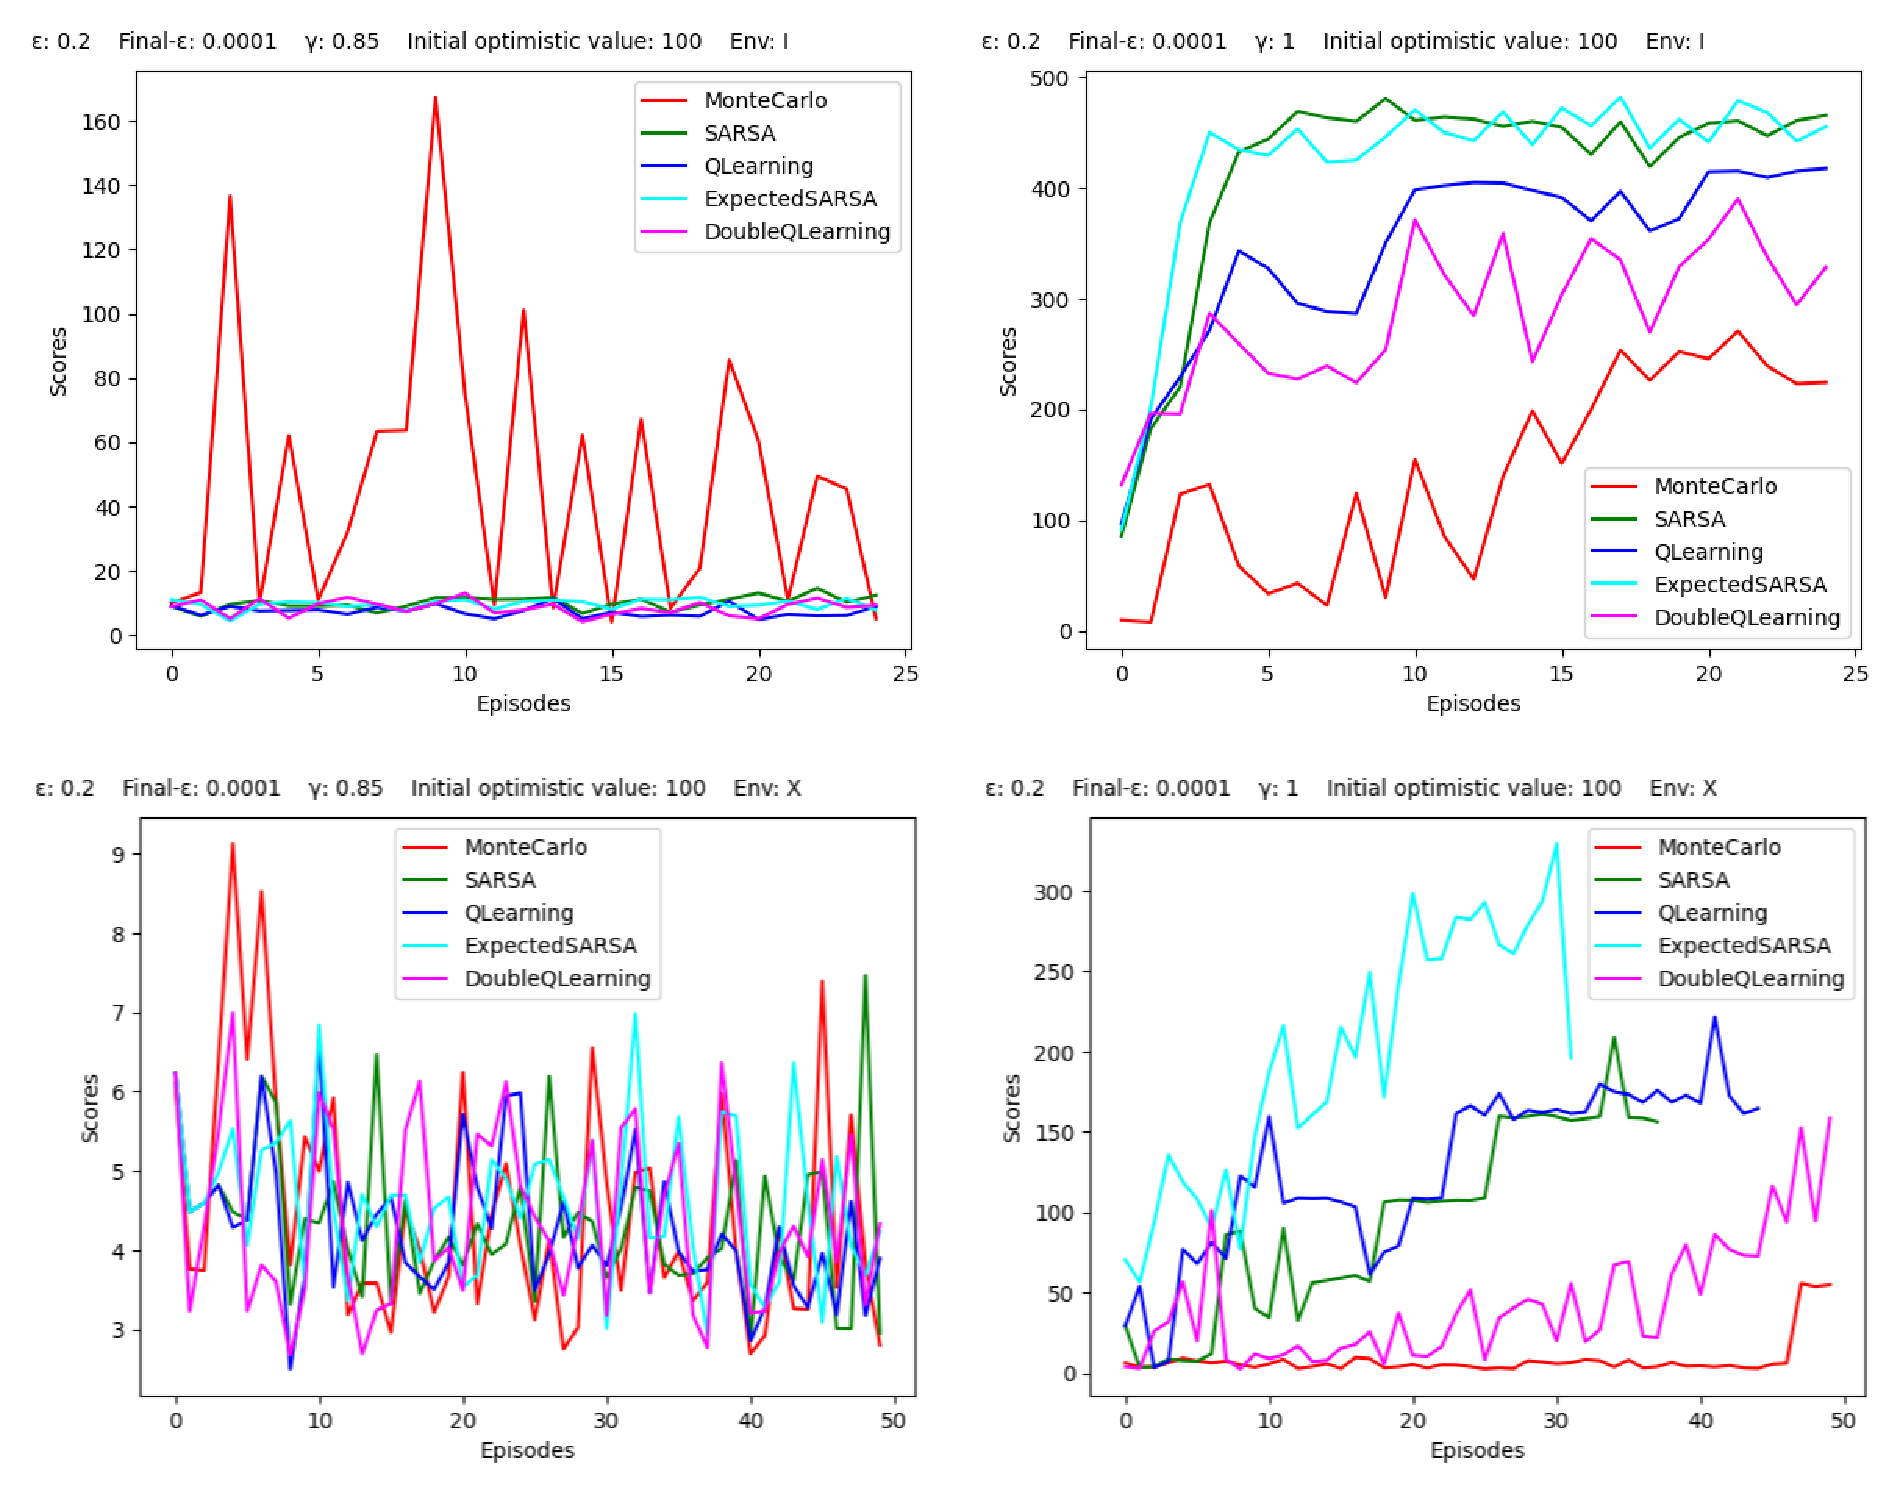
\includegraphics[width=\textwidth]{discountingExample}
    \caption{Discounting example}
    \label{fig:discounting_eg}
\end{figure}

In this chapter, we aim to discuss certain unexpected findings that surfaced during our experimentation. One of the immediate observations can be seen in Figure \ref{fig:discounting_eg}\footnote{No smoothing was applied to any of the plots in this subsection.}. We conducted experiments on two distinct environments, \texttt{env=[I]} and \texttt{env=[X]}, and for each environment, we carried out experiments with discount rates of \texttt{gam=0.85} and \texttt{gam=1.0} for all agents. As evident from the plots, the lower gamma value exhibited considerably poorer performance than when no discounting (\texttt{gam=1.0}) was applied. This trend is not limited to these specific environments and testing conditions but rather observed consistently across all our experimentation. This result is counter-intuitive since it seems logical that penalizing the last action more than previous ones would result in a better policy.

\begin{figure}[h]
    \centering
    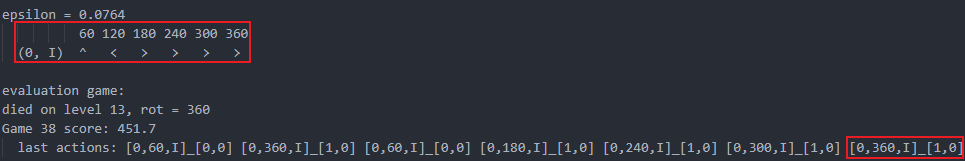
\includegraphics[width=\textwidth]{discountingExplanation}
    \caption{Discounting explanation}
    \label{fig:discounting_expl}
\end{figure}

Upon further investigation, we discovered that in some cases, a lost game for the agent does not result from the last action directly but rather from a chain reaction initiated by a previous bad decision. As seen in Figure \ref{fig:discounting_expl}, the agent's last action of going right at rotation \texttt{360} to reach a safe one, \texttt{60}, is not a poor decision in itself but rather the best possible action in that state\footnote{As confirmed by a human player, rotation 60 is safe for trap type I.}. However, analysing the last four actions taken by the agent, it becomes clear that it attempted to reach rotation \texttt{60} by going left from the rotation \texttt{180}. With a high score of \texttt{451.7} (Figure \ref{fig:discounting_eg}), the agent undeniably had high speed value, making it move forward very quickly, and while this policy may have been effective in the early game before the agent attained its current speed\footnote{It should recalled that after every 3 levels the agents speed increases.}, there is simply not enough time for the agent to rotate at this point in the game. In this case, one could argue that the fourth action from the last was responsible for the agent's loss. For cases like this, we believe that the agent performs better when all actions are penalized equally.

\begin{figure}[h]
    \centering
    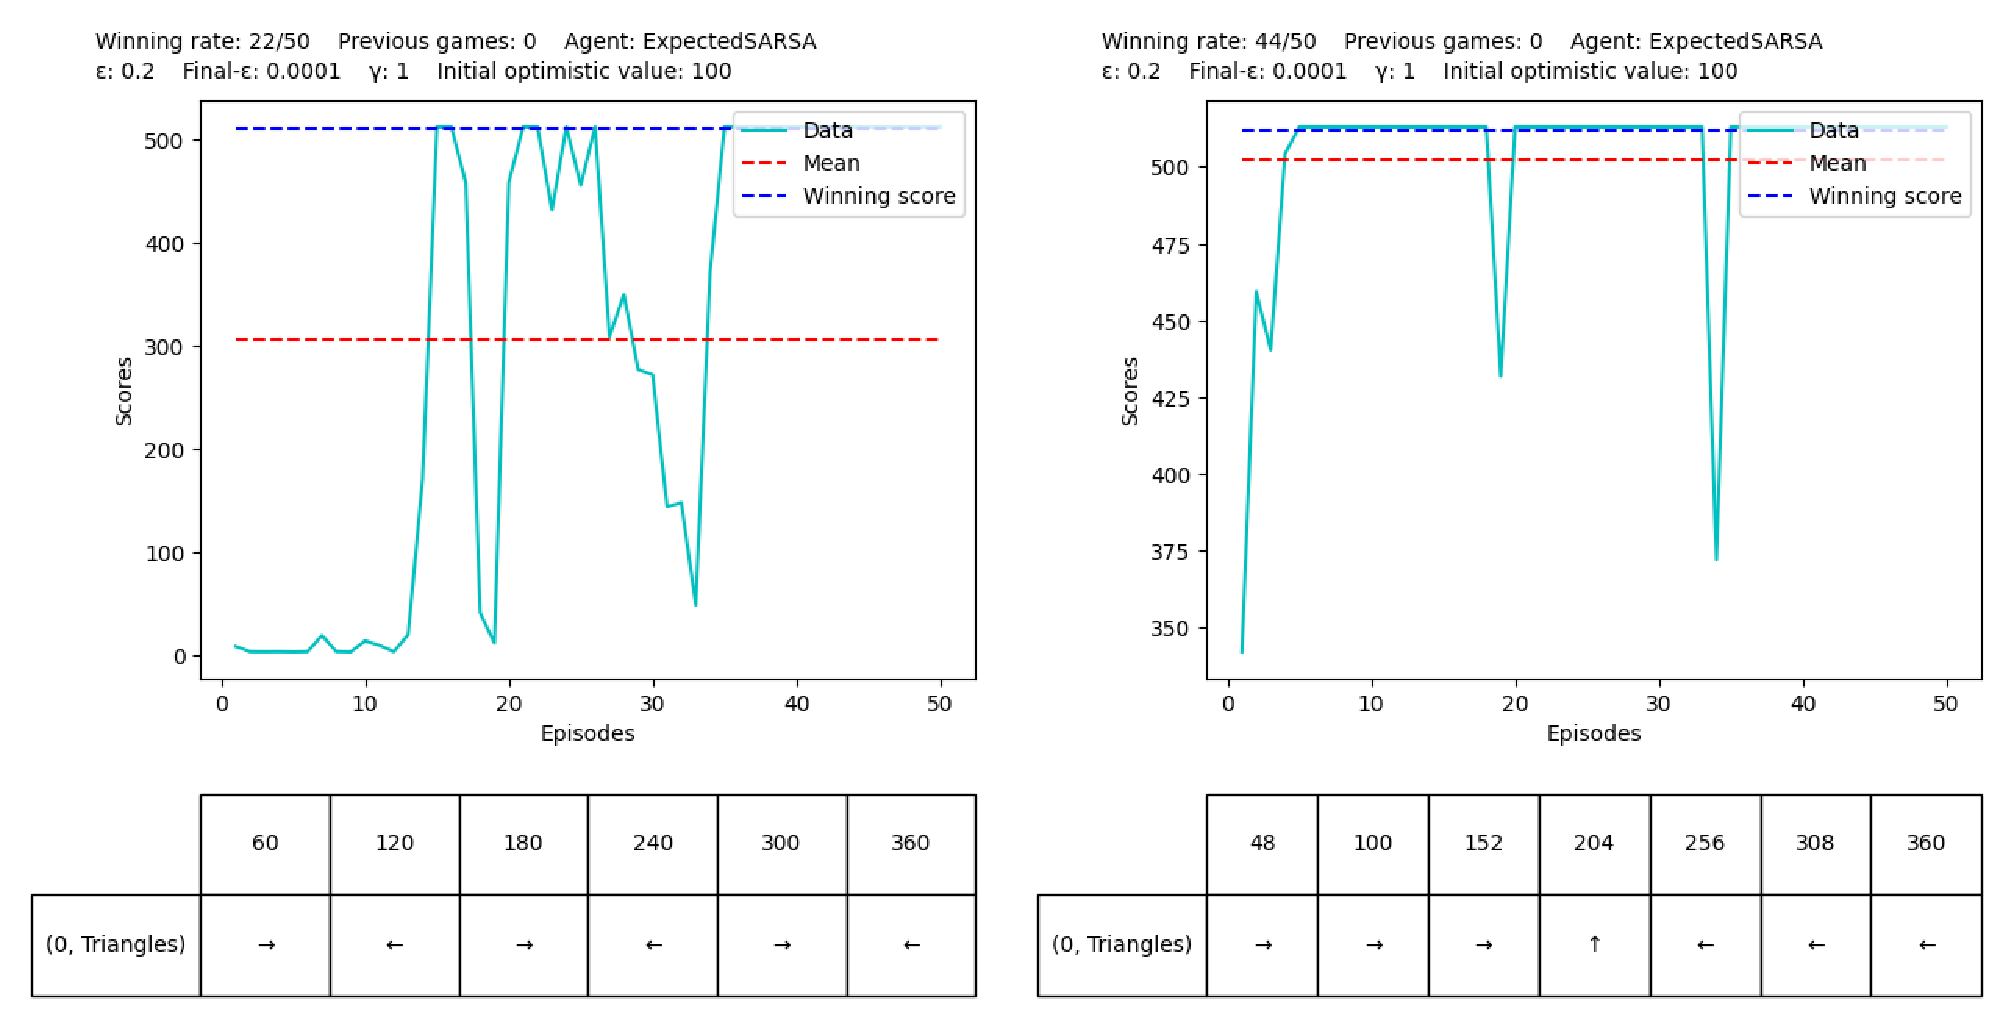
\includegraphics[width=\textwidth]{trianglesExample}
    \caption{\texttt{Triangles} example}
    \label{fig:triangles_intbeh_eg}
\end{figure}

Another intriguing behaviour emerged as a result of our learning architecture. As previously noted, we chose to have the agent not take a new action every time its \texttt{move()} function is called, but rather return the same action until the state changes. This resulted in a substantial reduction in the number of different actions taken by the agent, given that the move function is invoked every game tick, while state changes occur less frequently. This approach led to a behaviour that could not have been predicted at the outset. Figure \ref{fig:triangles_intbeh_eg} provides an illustration of this behaviour (with some sentiment \texttt{env=[Triangles]} was chosen as this was the first environment on which the behaviour was noticed).

Ordinarily, \texttt{env=[Triangles]} does not offer any safe rotations unless \texttt{rots=7} or more. As shown in the plot, the agent will certainly learn with this rotation value. However, if the agent is given only \texttt{6} rotation values to choose from, it will develop a policy that rapidly oscillates between two rotations, keeping the player character, Hans, on the edge of those rotations, allowing him to safely pass through the trap. This behaviour is not confined to situations where the agent is ``forced'' to make such a decision. During training, in many instances, the agent will learn to stay on the edge rather than advance into a completely safe rotation. There does not appear to be a preference for one or the other; rather, the policy the agent discovers first is determined by other experimental factors. It can be concluded that this behaviour arose solely because the agent did not alter its action until the state changed. In my opinion, this discovery is one of the most exciting outcomes of this project.
\chapter*{Conclusion}
\addcontentsline{toc}{chapter}{Conclusion}

%%% Bibliography
%%% Bibliography (literature used as a source)
%%%
%%% We employ bibTeX to construct the bibliography. It processes
%%% citations in the text (e.g., the \cite{...} macro) and looks up
%%% relevant entries in the bibliography.bib file.
%%%
%%% The \bibliographystyle command selects, which style will be used
%%% for references from the text. The argument in curly brackets is
%%% the name of the corresponding style file (*.bst). Both styles
%%% mentioned in this template are included in LaTeX distributions.

\bibliographystyle{plainnat}    %% Author (year)
% \bibliographystyle{unsrt}     %% [number]

\renewcommand{\bibname}{Bibliography}

%%% Generate the bibliography. Beware that if you cited no works,
%%% the empty list will be omitted completely.

\bibliography{bibliography}

%%% If case you prefer to write the bibliography manually (without bibTeX),
%%% you can use the following. Please follow the ISO 690 standard and
%%% citation conventions of your field of research.

% \begin{thebibliography}{99}
%
% \bibitem{lamport94}
%   {\sc Lamport,} Leslie.
%   \emph{\LaTeX: A Document Preparation System}.
%   2nd edition.
%   Massachusetts: Addison Wesley, 1994.
%   ISBN 0-201-52983-1.
%
% \end{thebibliography}


%%% Figures used in the thesis (consider if this is needed)
\listoffigures

%%% Tables used in the thesis (consider if this is needed)
%%% In mathematical theses, it could be better to move the list of tables to the beginning of the thesis.
\listoftables

%%% Abbreviations used in the thesis, if any, including their explanation
%%% In mathematical theses, it could be better to move the list of abbreviations to the beginning of the thesis.
\chapwithtoc{List of Abbreviations}

%%% Attachments to the bachelor thesis, if any. Each attachment must be
%%% referred to at least once from the text of the thesis. Attachments
%%% are numbered.
%%%
%%% The printed version should preferably contain attachments, which can be
%%% read (additional tables and charts, supplementary text, examples of
%%% program output, etc.). The electronic version is more suited for attachments
%%% which will likely be used in an electronic form rather than read (program
%%% source code, data files, interactive charts, etc.). Electronic attachments
%%% should be uploaded to SIS and optionally also included in the thesis on a~CD/DVD.
%%% Allowed file formats are specified in provision of the rector no. 72/2017.
\appendix
\chapter{Attachments}

\section{First Attachment}

\openright
\end{document}
